\section{问题求解}
\subsection{开发环境搭建}
\begin{itemize}
  \item 安装 JDK8(GeaFlow 目前只支持 JDK8), 包括配置相应的环境变量.
  \item 安装 Maven, 包括配置相应的环境变量.
  \item 安装任意可以编写代码的文本编辑器.
  \item 下载数据集到本地磁盘.
\end{itemize}

添加 Maven 坐标(完整配置可见项目源码的 pom.xml 文件):
\begin{center}
\begin{minted}[xleftmargin=5mm]{xml}
<dependency>
    <groupId>com.antgroup.tugraph</groupId>
    <artifactId>geaflow-api</artifactId>
    <version>0.3</version>
</dependency>

<dependency>
    <groupId>com.antgroup.tugraph</groupId>
    <artifactId>geaflow-pdata</artifactId>
    <version>0.3</version>
</dependency>

<dependency>
    <groupId>com.antgroup.tugraph</groupId>
    <artifactId>geaflow-cluster</artifactId>
    <version>0.3</version>
</dependency>

<dependency>
    <groupId>com.antgroup.tugraph</groupId>
    <artifactId>geaflow-on-local</artifactId>
    <version>0.3</version>
</dependency>

<dependency>
    <groupId>com.antgroup.tugraph</groupId>
    <artifactId>geaflow-pipeline</artifactId>
    <version>0.3</version>
</dependency>
\end{minted}
\end{center}

打包:
\begin{center}
\begin{minted}[xleftmargin=5mm]{bash}
mvn clean package -DskipTests
\end{minted}
\end{center}

运行:
\begin{center}
\begin{minted}[xleftmargin=5mm]{bash}
$JAVA_HOME/bin/java -jar target/*.jar 数据集路径 结果文件路径
\end{minted}
\end{center}

\subsection{通用的类和函数}
由于问题是基于 GeaFlow API 进行图构建和计算的, 对于不同的问题,
仅仅是点和边的数据发生改变, 构图的 API 是相似的, 为此我们抽象出
求解各个问题的通用类和函数.

\subsubsection{图输入}
具体输入数据的格式可见问题描述一节, 此处不再赘述.
相关依赖的导入请见相关源码文件, 此处为避免篇幅过长, 故省略之.

\begin{center}
\begin{minted}[xleftmargin=5mm]{java}
package org.graphpatmatch.yyds.utils;

public class FileSource<OUT>
  extends RichFunction implements SourceFunction<OUT> {
  // 文件名
  protected String filePath;
  // 输入文件的路径
  public static final String INPUT_DIR = "input.dir";
  // 读入的数据
  protected List<OUT> records;
  protected Integer readPos = null;
  // 读入数据的解析器
  protected FileLineParser<OUT> parser;
  protected transient RuntimeContext runtimeContext;

  public FileSource(String filePath, FileLineParser<OUT> parser) {
    this.filePath = filePath;
    this.parser = parser;
  }

  @Override
  public void open(RuntimeContext runtimeContext) {
    this.runtimeContext = runtimeContext;
    filePath = String.format("%s/%s",
        runtimeContext.getConfiguration().getString("input.dir"), filePath);
  }

  @Override
  public void init(int parallel, int index) {
    this.records = readFileLines(filePath);
    if (parallel != 1) {
      List<OUT> allRecords = records;
      records = new ArrayList<>();
      for (int i = 0; i < allRecords.size(); i++) {
        if (i % parallel == index) {
          records.add(allRecords.get(i));
        }
      }
    }
  }

  @Override
  public boolean fetch(IWindow<OUT> window, SourceContext<OUT> ctx)
    throws Exception {
    if (readPos == null) {
      readPos = 0;
    }
    while (readPos < records.size()) {
      OUT out = records.get(readPos);
      long windowId = window.assignWindow(out);
      if (window.windowId() == windowId) {
        ctx.collect(out);
        readPos++;
      } else {
        break;
      }
    }
    boolean result = false;
    if (readPos < records.size()) {
      result = true;
    }
    return result;
  }

  // 以行为单位读入数据
  private List<OUT> readFileLines(String filePath) {
    try {
      List<String> lines = Files.readLines(new File(filePath),
          Charset.defaultCharset());
      List<OUT> result = new ArrayList<>();

      // 过滤掉首行(header)
      lines.remove(0);

      for (String line : lines) {
        if (StringUtils.isBlank(line)) {
          continue;
        }
        Collection<OUT> collection = parser.parse(line);
        result.addAll(collection);
      }
      return result;
    } catch (IOException e) {
      throw new RuntimeException("error in read resource file: " + filePath, e);
    }
  }

  public interface FileLineParser<OUT> extends Serializable {
    Collection<OUT> parse(String line);
  }
}
\end{minted}
\end{center}

\subsubsection{图输出}
\begin{center}
\begin{minted}[xleftmargin=5mm]{java}
package org.graphpatmatch.yyds.utils;

public class FileSink<OUT>
  extends RichFunction implements SinkFunction<OUT> {
  // 输出文件路径
  public static final String OUTPUT_DIR = "output.dir";
  // 输出文件名
  public static final String OUTPUT_FILE = "output.file";
  public static final String FILE_OUTPUT_APPEND_ENABLE = "file.append.enable";
  private Boolean first = false;
  private File file;

  public FileSink() {
  }

  @Override
  public void open(RuntimeContext runtimeContext) {
    String filePath = String.format("%s/%s",
        runtimeContext.getConfiguration().getString(OUTPUT_DIR),
        runtimeContext.getConfiguration().getString(OUTPUT_FILE));

    boolean append = runtimeContext.getConfiguration()
      .getBoolean(new ConfigKey(FILE_OUTPUT_APPEND_ENABLE, true));
    file = new File(filePath);

    // 若指定的文件不存在, 则创建之
    try {
      if (!append && file.exists()) {
        try {
          FileUtils.forceDelete(file);
        } catch (Exception e) {
          // ignore
        }
      }

      if (!file.exists()) {
        if (!file.getParentFile().exists()) {
          file.getParentFile().mkdirs();
        }
        file.createNewFile();
      }
    } catch (IOException e) {
      throw new GeaflowRuntimeException(e);
    }
  }

  @Override
  public void write(OUT out) throws Exception {
    try {
      // 写入首行(header)
      if (!first) {
        FileUtils.write(file, "id|value\n", Charset.defaultCharset(), true);
        first = true;
      }
      // 逐行写入
      FileUtils.write(file, out + "\n", Charset.defaultCharset(), true);
    } catch (IOException e) {
      throw new RuntimeException(e);
    }
  }
}
\end{minted}
\end{center}

\subsubsection{输出排序}
结果文件要求输出按照 id 的数值大小进行升序排序, 我们在此处说明排序的逻辑.

\begin{center}
\begin{minted}[xleftmargin=5mm]{java}
package org.graphpatmatch.yyds.utils;

public class FileSort {
  public static void sort(String TMP_FILE, String RESULT_FILE) {
    try {
      // 中间文件
      File fin = new File(TMP_FILE);
      // 结果文件
      File fout = new File(RESULT_FILE);

      FileInputStream fis = new FileInputStream(fin);
      FileOutputStream fos = new FileOutputStream(fout);

      BufferedReader in = new BufferedReader(new InputStreamReader(fis));
      BufferedWriter out = new BufferedWriter(new OutputStreamWriter(fos));

      String aLine;
      // 有序映射, <id, value>: <BigInteger, String>
      SortedMap<BigInteger, String> sortedMap = new TreeMap<BigInteger, String>();

      in.readLine(); // Skip the first line(header)
      while ((aLine = in.readLine()) != null) {
        if (aLine.trim().length() > 0) { // 非空行
          // split() 根据正则表达式进行分割, | 是正则表达式的元字符, 故需转义
          sortedMap.put(new BigInteger(aLine.split("\\|")[0]), aLine);
        }
      }

      out.write("id|value\n"); // Write header
      Set<Entry<BigInteger, String>> entries = sortedMap.entrySet();
      for (Entry<BigInteger, String> entry : entries) {
        out.write(entry.getValue() + "\n");
      }

      in.close();
      out.close();
      // 删除临时文件
      FileUtils.forceDelete(new File(TMP_FILE));
    } catch (IOException e) {
    }
  }
}
\end{minted}
\end{center}

程序运行时环境的初始化和参数配置请见源码, 以下仅描述
构图过程和核心算法.

\subsection{交易闭环搜索问题}
具体问题描述可见 \ref{pro1} 交易闭环搜索问题 一节.

此问题涉及的数据文件有:
\begin{itemize}
  \item Account.csv(点)
  \item AccountTransferAccount.csv(边)
\end{itemize}

\subsubsection{输入}
\begin{center}
\begin{minted}[xleftmargin=5mm]{java}
// 构建点
PWindowSource<IVertex<String, Integer>> vertices = pipelineTaskCxt
  .buildSource(
    new FileSource<IVertex<String, Integer>>(
      "Account.csv",
      line -> {
        String[] fields = line.split("\\|");
        // <vertexKey, vertexValue>: <String, Integer>
        // 此处以 Account 的 Id 作为点的 Id,
        // 点的值为以此点为源点的三角形的个数
        IVertex<String, Integer> vertex = new ValueVertex<String, Integer>(
        fields[0], 0);
        return Collections.singletonList(vertex);
    }),
    AllWindow.getInstance())
  .withParallelism(sourceParallelism);

// 构建边
PWindowSource<IEdge<String, String>> edges = pipelineTaskCxt
  .buildSource(
    new FileSource<IEdge<String, String>>(
      "AccountTransferAccount.csv",
      line -> {
        String[] fields = line.split("\\|");
        // <vertexKey, edgeValue>: <String, String>
        // 此处以 Account 的 Id 作为点的 Id
        IEdge<String, String> edge = new ValueEdge<String, String>(
          fields[0], fields[1], ""); // (srcId, targetId, edgeValue)
        return Collections.singletonList(edge);
    }),
    AllWindow.getInstance())
  .withParallelism(sourceParallelism);

// 构造图视图(用于将构造出的点和边关联起来)
GraphViewDesc graphViewDesc = GraphViewBuilder
  .createGraphView(GraphViewBuilder.DEFAULT_GRAPH)
  .withShardNum(iterationParallelism)
  .withBackend(BackendType.Memory)
  .build();
\end{minted}
\end{center}

\subsubsection{核心算法}
此问题可看作是寻找图中三角形 $ K^{3} $ 的个数.

对图中的某个点 $ A $, $ A $ 向每个相邻点发送消息 $ M=(1, A) $, 此后消息
$ M $ 每传递一次, $ M $ 的第一个元素的值就增加 $ 1 $, 若 $ A $ 在某个三角形中,
则 $ M $ 最终会被传回给 $ A $, 此时 $ M = (3, A) $, 点 $ A $
发现这是自己发出的消息, 于是更新状态(以 $ A $ 为源点的三角形个数);
若 $ M $ 的第一个元素的值为 $ 3 $ 且消息到达的点的 Id 与 $ M $ 的第二个元素不等,
则丢弃该消息, 不再继续传递.

\begin{figure}[H]
  \begin{center}
    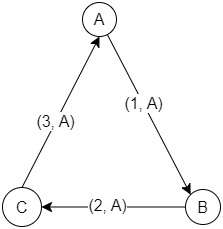
\includegraphics[width=0.15\textwidth]{./figures/pro1.jpg}
  \end{center}
  \caption{交易闭环搜索消息传递}
\end{figure}

\begin{center}
\begin{minted}[xleftmargin=5mm]{java}
public void compute(
  String vertexId, Iterator<String> messageIterator) {
  IVertex<String, Integer> vertex = this.context.vertex().get();

  // 首轮迭代向所有相邻节点发送消息
  if (this.context.getIterationId() == 1L) {
    this.context.sendMessageToNeighbors("1," + vertexId);
  }

  while (messageIterator.hasNext()) {
    String[] msg = messageIterator.next().split(",");
    int t = Integer.parseInt(msg[0]);
    String msgId = msg[1];

    if (t < 3) {
      t += 1;
      if (t == 3) {
        List<IEdge<String, String>> edges = this.context
          .edges().getOutEdges();
        for (IEdge<String, String> edge : edges) {
          if (msgId.equals(edge.getTargetId())) {
            // 仅向可以形成闭环的点发送消息,
            // 避免非必要的内存浪费和减少计算的时间开销
            this.context.sendMessage(msgId, "3," + msgId);
          }
        }
      } else {
        this.context.sendMessageToNeighbors(
          Integer.toString(t) + "," + msgId);
      }
    } else if (t == 3) { // 找到一个闭环, 更新结果
      this.context.setNewVertexValue(vertex.getValue() + 1);
    }
  }
}
\end{minted}
\end{center}

\subsubsection{输出}
\begin{center}
\begin{minted}[xleftmargin=5mm]{java}
PWindowStream<IVertex<String, Integer>> result = pipelineTaskCxt
  .buildWindowStreamGraph(vertices, edges, graphViewDesc)
  .compute(new Case2Algorithms(4)) // 迭代 4 轮
  .compute(iterationParallelism)
  .getVertices();

SinkFunction<String> sink = ExampleSinkFunctionFactory
  .getSinkFunction(conf);
result
  .filter(v -> v.getValue() >= 1) // 过滤出符合要求的点
  .map(v -> String.format("%s|%s", v.getId(), v.getValue()))
  .withParallelism(mapParallelism)
  .sink(sink) // 写入文件
  .withParallelism(sinkParallelism);
\end{minted}
\end{center}

\subsection{资金快进快出问题}
具体问题描述可见 \ref{pro2} 资金快进快出问题一节.

此问题涉及的数据文件有:
\begin{itemize}
  \item Account.csv(点)
  \item AccountTransferAccount.csv(边)
\end{itemize}

\subsubsection{输入}
\begin{center}
\begin{minted}[xleftmargin=5mm]{java}
// 构建点
PWindowSource<IVertex<String, String>> vertices = pipelineTaskCxt
  .buildSource(
    new FileSource<IVertex<String, String>>(
      "Account.csv",
      line -> {
        String[] fields = line.split("\\|");
        // <vertexKey, vertexValue>: <String, String>
        // 此处以 Account 的 Id 作为点的 Id,
        IVertex<String, String> vertex = new ValueVertex<String, String>(
          fields[0], "");
        return Collections.singletonList(vertex);
    }),
    AllWindow.getInstance())
  .withParallelism(sourceParallelism);

// 构建边
PWindowSource<IEdge<String, Double>> edges = pipelineTaskCxt
  .buildSource(
    new FileSource<IEdge<String, Double>>(
      "AccountTransferAccount.csv",
      line -> {
        String[] fields = line.split("\\|");
        // <vertexKey, edgeValue>: <String, Double>
        // 此处以 Account 的 Id 作为点的 Id
        IEdge<String, Double> edge = new ValueEdge<String, Double>(
          fields[0], fields[1], Double.parseDouble(fields[2]));
        // (srcId, targetId, edgeValue)
        return Collections.singletonList(edge);
      }),
      AllWindow.getInstance())
  .withParallelism(sourceParallelism);

// 构造图视图(用于将构造出的点和边关联起来)
GraphViewDesc graphViewDesc = GraphViewBuilder
  .createGraphView(GraphViewBuilder.DEFAULT_GRAPH)
  .withShardNum(iterationParallelism)
  .withBackend(BackendType.Memory)
  .build();
\end{minted}
\end{center}

\subsubsection{核心算法}

此问题中涉及到的图记作 $ G $, 对一个点 $ v \in V(G) $,
\begin{enumerate}
  \item 找到 $ v $ 的所有入边 $ wv \in E(G), w \in V(G) $(至少一条),
    对所有入边的值求和 $ M=\sum_{i=1}^{m} val(w_iv) $, 其中的 $ m $ 是 $ v $
    的入边的数量, $ val(w_iv) $ 是 $ v $ 的入边 $ w_iv $ 的值;
  \item 找到 $ v $ 的所有出边 $ vx \in E(G), x \in V(G) $(至少一条),
    对所有出边的值求和 $ N=\sum_{j=1}^{n} val(vx_j)$, 其中 $ n $ 是 $ v $
    的出边的数量, $ val(vx_i) $ 是 $ v $ 的出边 $ vx_i $ 的值;
  \item 得到结果 $ M / N $.
\end{enumerate}

\begin{center}
\begin{minted}[xleftmargin=5mm]{java}
public void compute(
  String vertexId, Iterator<Double> messageIterator) {
  List<IEdge<String, Double>> edges = this.context.edges().getOutEdges();

  // 第一轮迭代向所有出边的目标点发送边值
  if (this.context.getIterationId() == 1L) {
    for (IEdge<String, Double> edge : edges) {
      this.context.sendMessage(edge.getTargetId(), edge.getValue());
    }
  } else {
    // 第二轮迭代接收发来的信息
    double in_sum = 0.0, out_sum = 0.0;

    while (messageIterator.hasNext()) {
      Double msg = messageIterator.next();
      in_sum += msg;
    }
    if (in_sum == 0.0)
      return;

    for (IEdge<String, Double> edge : edges) {
      out_sum += edge.getValue();
    }
    if (out_sum != 0.0) {
      double res = in_sum / out_sum;
      String resStr = "";
      resStr = String.format("%.2f", res);
      this.context.setNewVertexValue(resStr);
    }
  }
}
\end{minted}
\end{center}

\subsubsection{输出}
\begin{center}
\begin{minted}[xleftmargin=5mm]{java}
PWindowStream<IVertex<String, String>> result = pipelineTaskCxt
  .buildWindowStreamGraph(vertices, edges, graphViewDesc)
  .compute(new Case3Algorithms(2)) // 进行 2 轮迭代
  .compute(iterationParallelism)
  .getVertices();

SinkFunction<String> sink = ExampleSinkFunctionFactory.getSinkFunction(conf);
result
  .filter(v -> !v.getValue().equals("")) // // 过滤出符合要求的点
  .map(v -> String.format("%s|%s", v.getId(), v.getValue()))
  .withParallelism(mapParallelism)
  .sink(sink) // 写入文件
  .withParallelism(sinkParallelism);
\end{minted}
\end{center}

\subsection{担保金额汇总问题}
具体问题描述可见 \ref{pro3} 担保金额汇总问题一节.

备注: 此问题我们花了大量时间与精力,但是没有解决,我们进行了两次修改,但都以失
败告终,但是仍有很大收获。

此问题涉及的数据文件有:
\begin{itemize}
  \item Person.csv(点)
  \item Loan.csv(点)
  \item PersonApplyLoan.csv(边)
  \item PersonGuarantee.csv(边)
\end{itemize}

\subsubsection{思路历程}
根据题目需分两步走,首先我们需要知道 person 所 guarantee 的 person 的 loan
的 amount 信息,所以,我们打算先将 Person.csv 和 Loan.csv 与 PersonApplyLoan 连接起来,
得出一张包含 personid 和此 person 所 apply 的 loan 的 amount 总和两个字段的新表,接着第二步,
根据这张新表与 personguaranteeperson 表,再去分析 person 下游的人找到满足要求的
person 信息。

\subsubsection{代码分析与实现}
由于在此项目中,分为点文件和边文件,可以抽象理解为根据输入的点和边,点具有 id 和
value 两个属性,边具有起始点 id 和终点 id 和 value 三个属性,调用接口后为抽象成一幅图,
可以对图(所有点)进行迭代,遍历等操作。于是,我们先将person和loan都当作点,点
的 id 即为 person 或 loan 对应的 id,而对于 value 值,我们将 loan 的 value 设为其 amount,将
person的value设为0,对于边,将value设置为空字符串,通过输入流 pwindowsource 分别
进行输入。接着我们用 buildwindowstreamgraph 进行构图,在构图中我们用 union 操作将
loan 和 person 点合并在一起,代码如下:
\begin{figure}[H]
  \begin{center}
    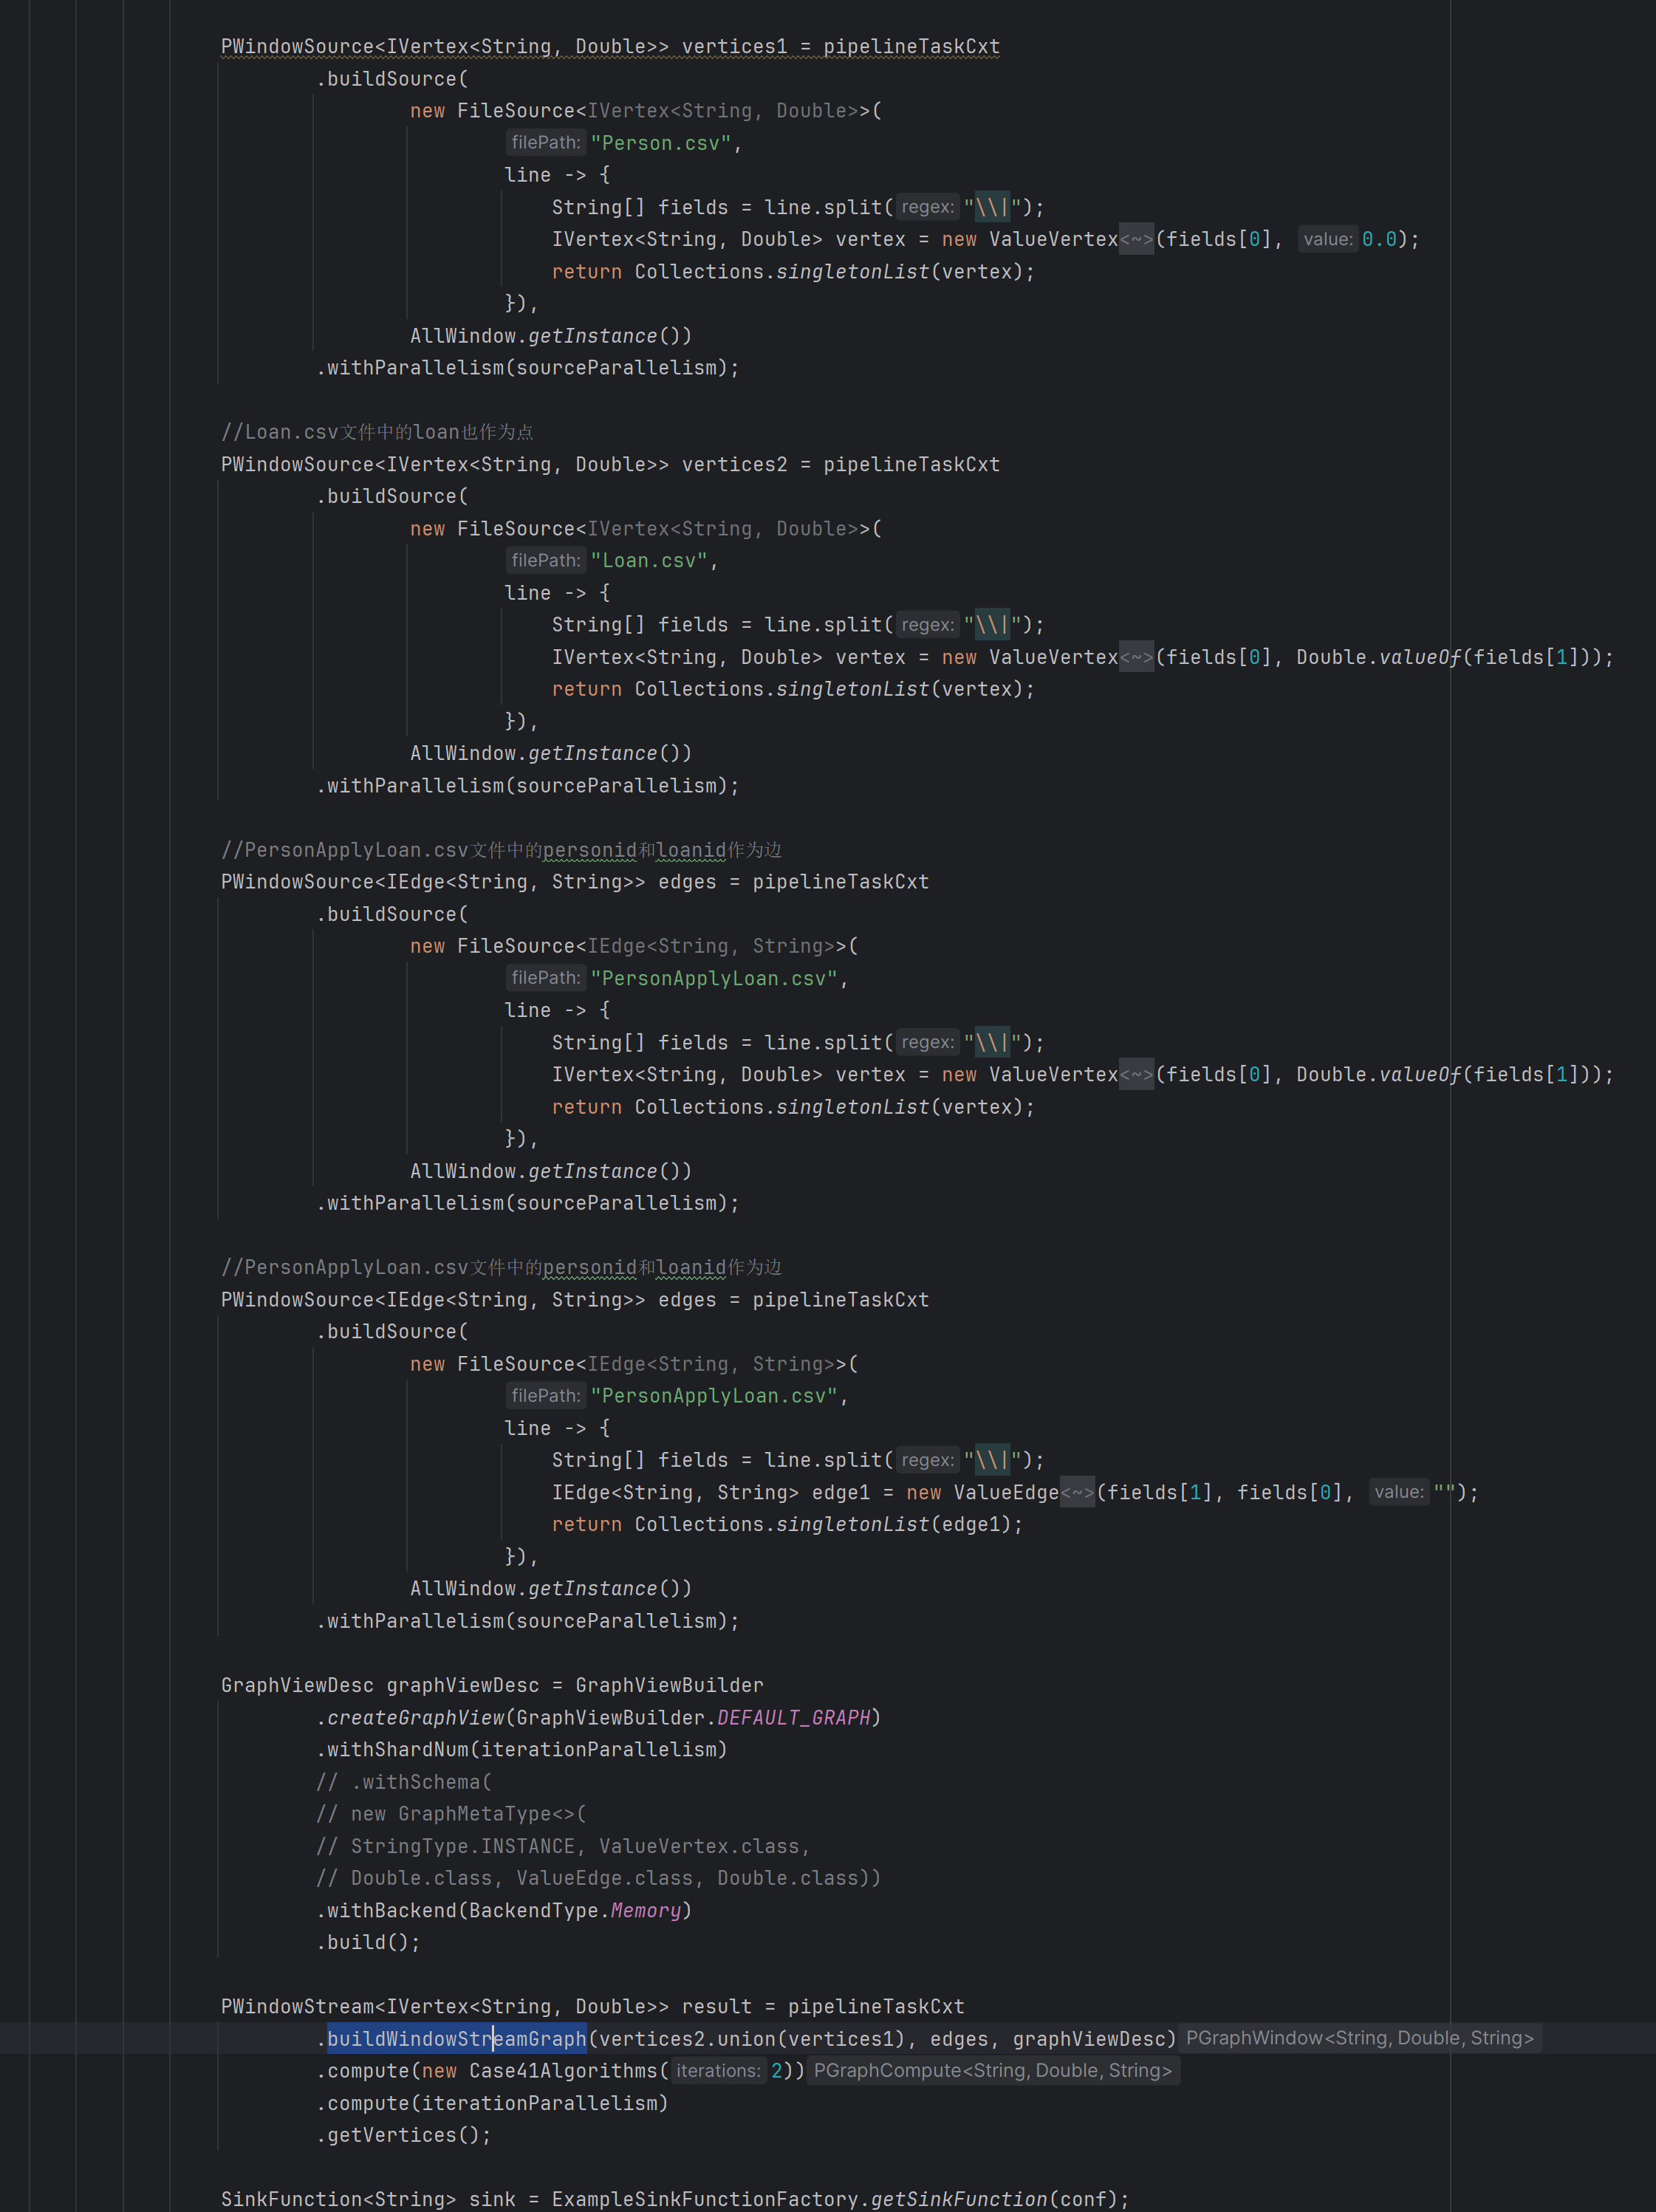
\includegraphics[width=0.85\textwidth,scale=0.7]{./figures/pro3/1.png}
  \end{center}
\end{figure}

接着我们需要得出一个新文件让每个person带上amount,于是,算法思路是进行对所有点
进行两轮迭代,第一轮所有点迭代中,让所有拥有出边的loan点(即此loan有至少一个人
apply),向所有出边的目标点(即person点)发送自己的amount值。最后将自己的value
值设置为 $ -1 $
以方便后续的过滤。(区分person点和loan点的方式是value值是否大于0)

在第二轮迭代中,由于每个点都有一个接收器,我们让所有接收器不为空的点(即person点)
计算接收器的总和 sum 并将 value 值更新为 sum,
到这一步,所有 person 的 value 值 $ >=0 $,所有 loan 的 value 值都为 $ -1 $,
核心代码如下:
\begin{figure}[H]
  \begin{center}
    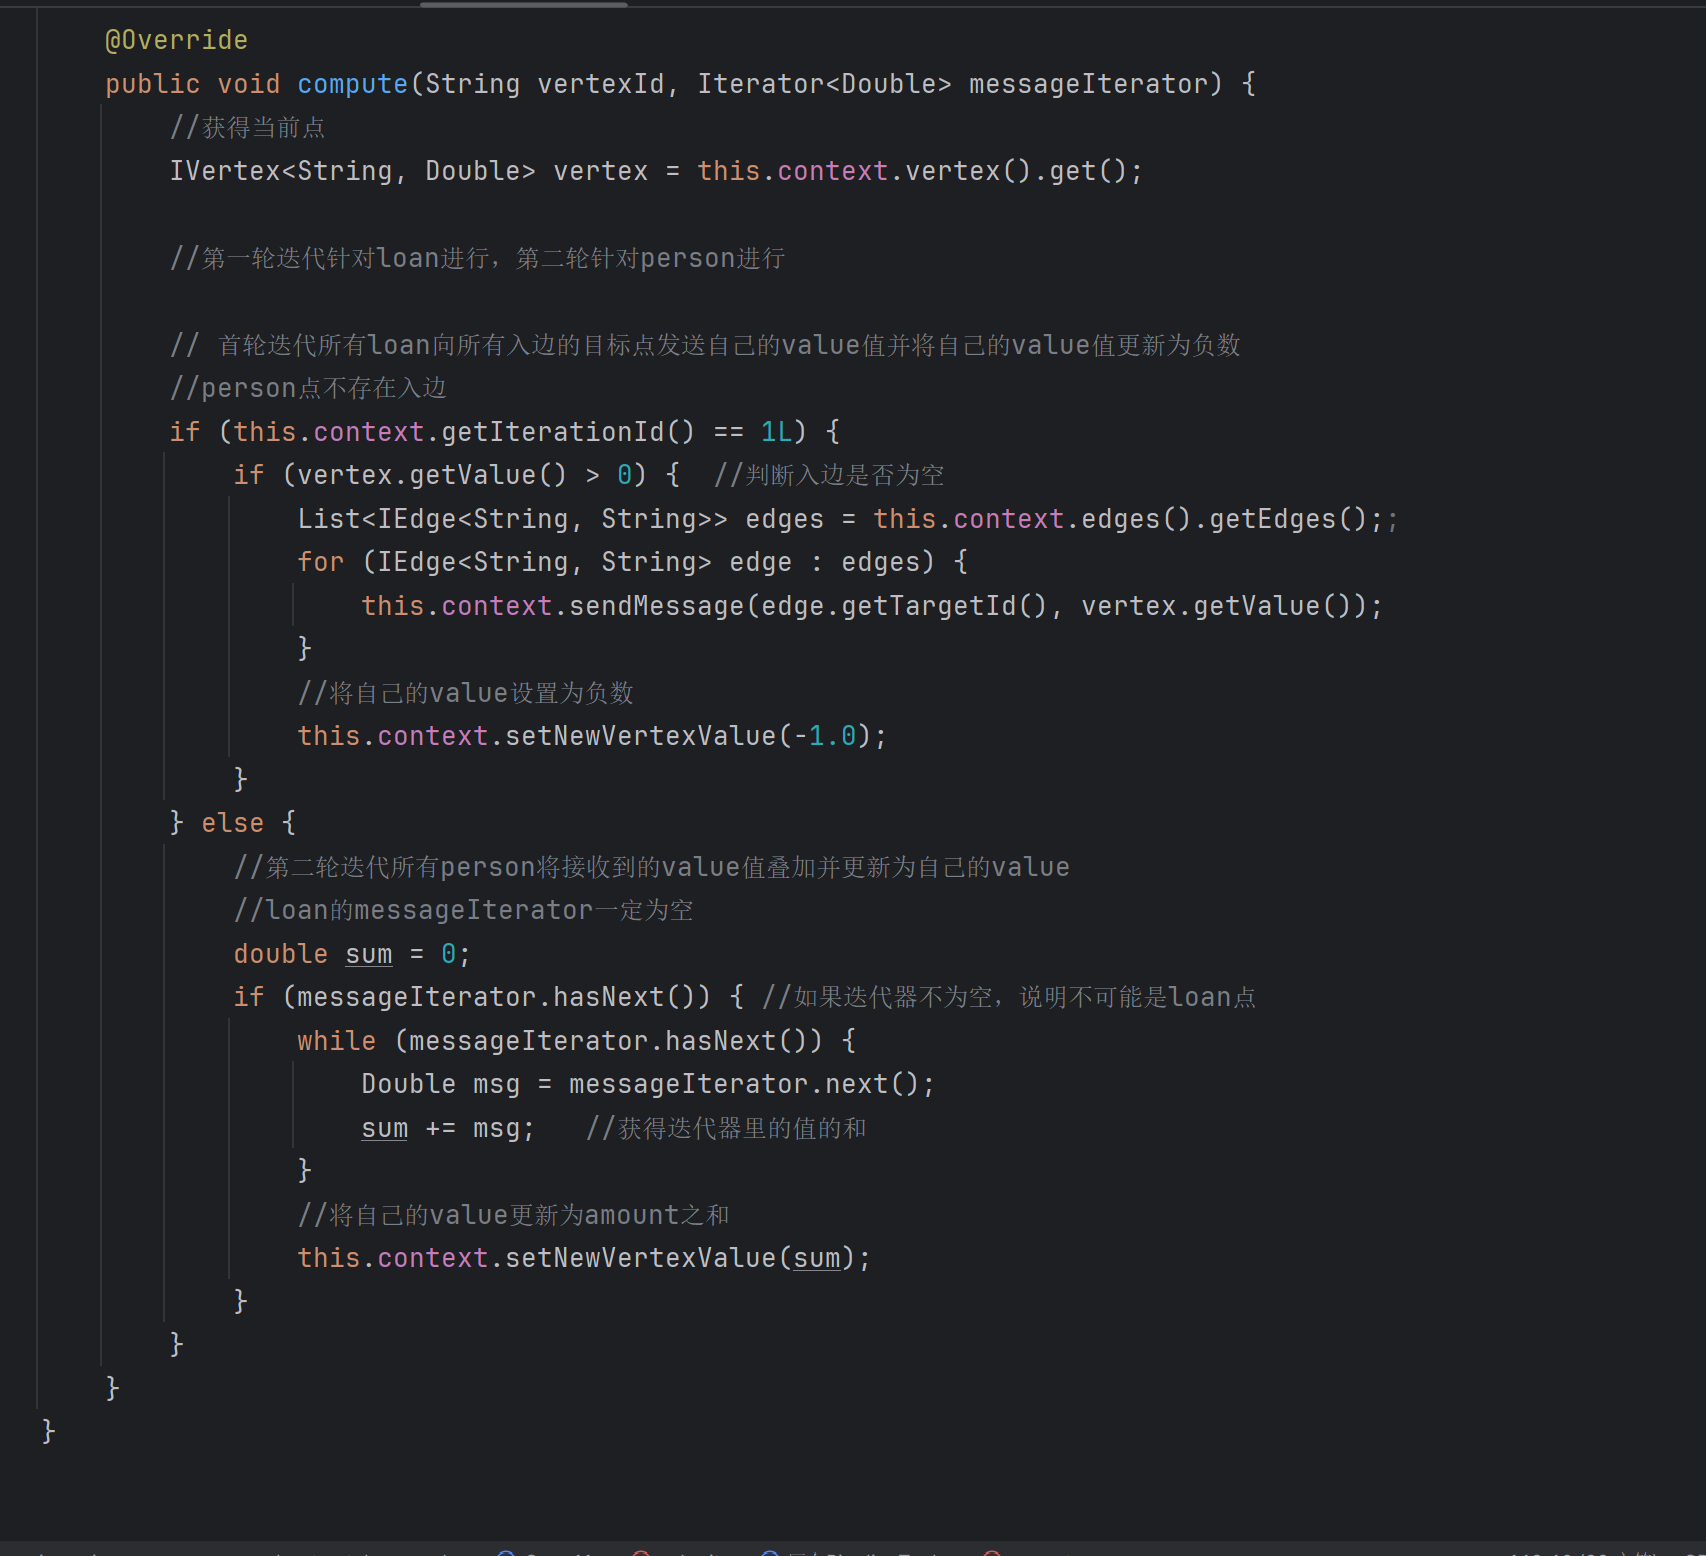
\includegraphics[width=0.85\textwidth,scale=0.7]{./figures/pro3/2.png}
  \end{center}
\end{figure}

最后,将所有点进行过滤涤除value 小于 $ 0 $ 的点(即loan点)得到中间文件。
\begin{figure}[H]
  \begin{center}
    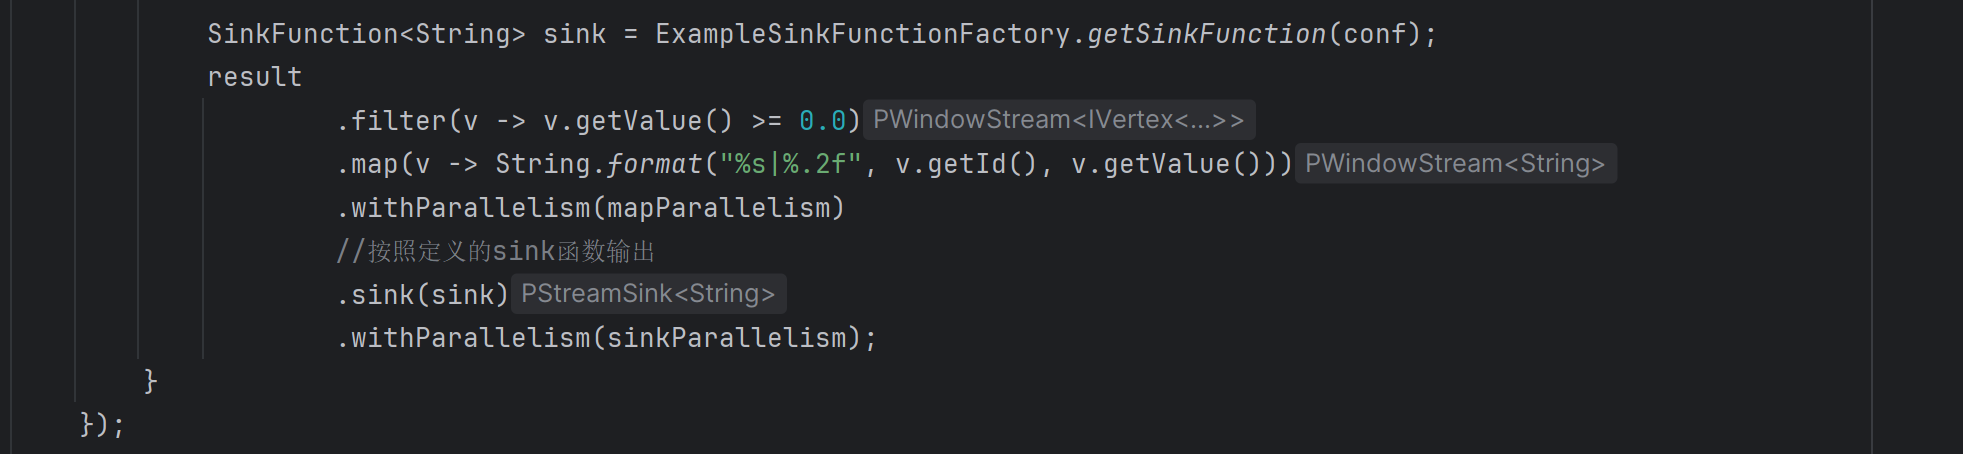
\includegraphics[width=0.85\textwidth,scale=0.7]{./figures/pro3/3.png}
  \end{center}
\end{figure}

接着进入第二步操作,首先因为我们要将中间文件与personguaranteeperson文件联合起来
构建成图,点的id为person的id,点的value为person的value,边的value为空字符串:
\begin{figure}[H]
  \begin{center}
    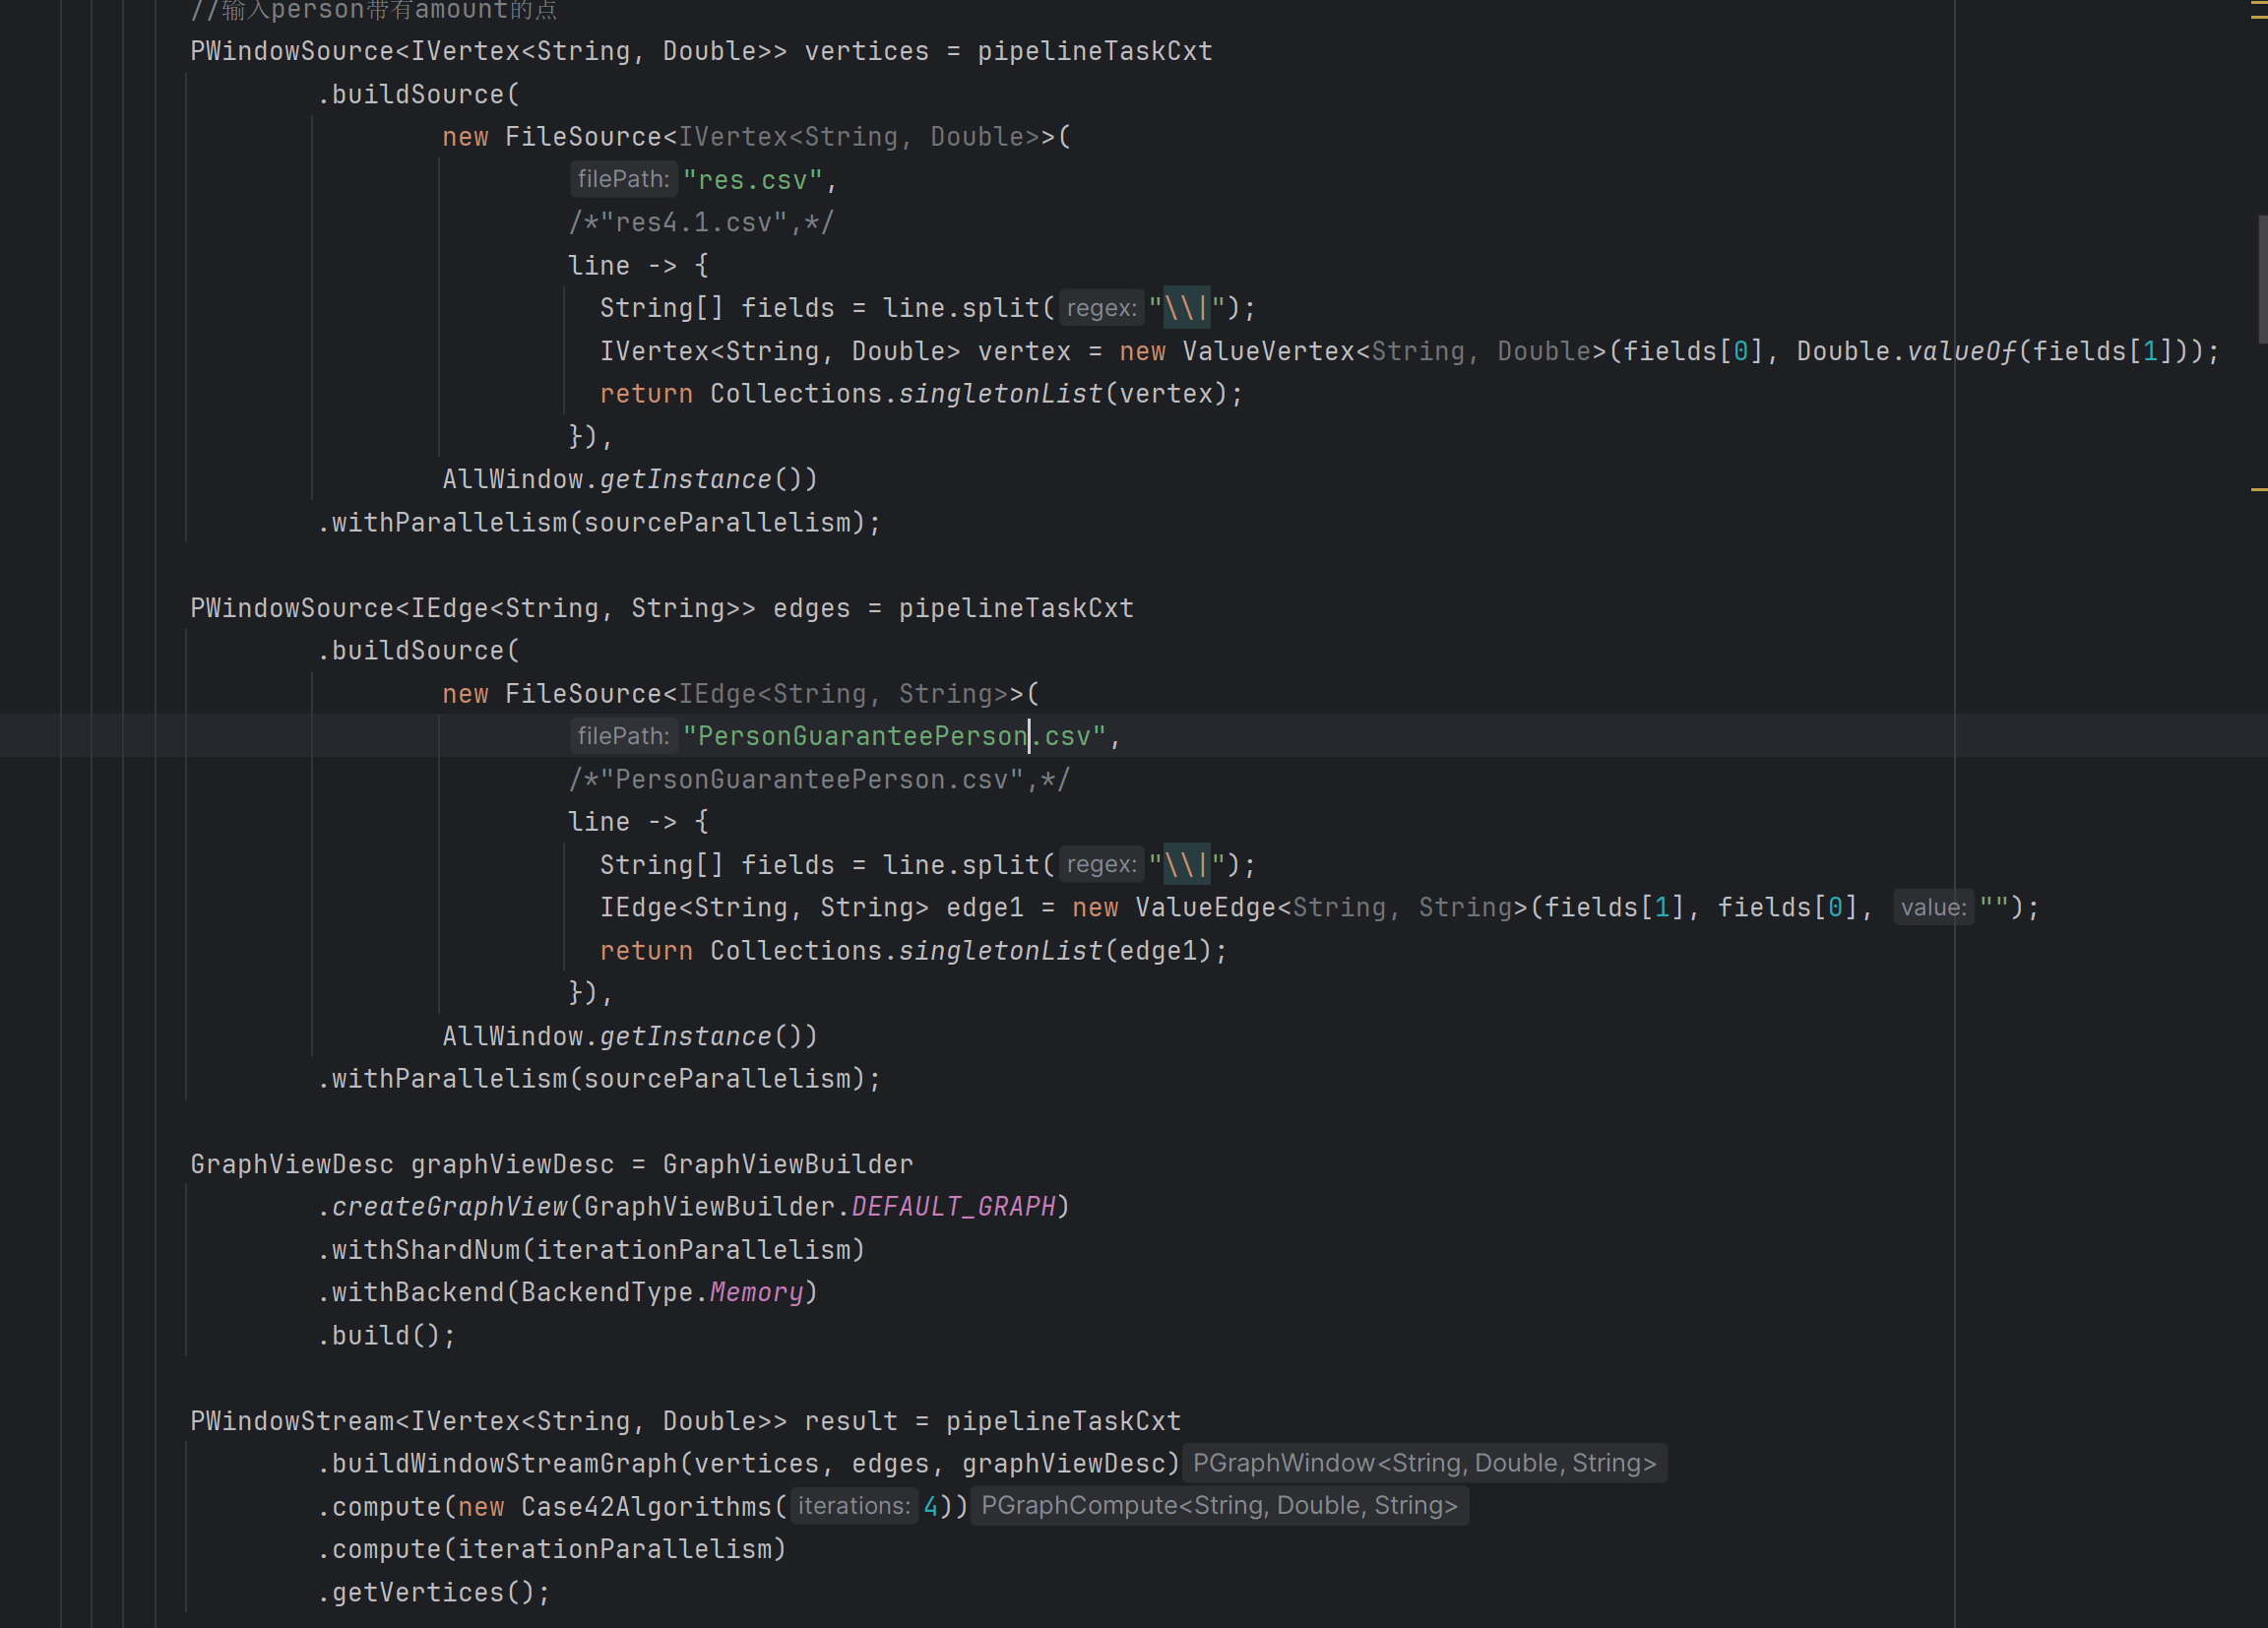
\includegraphics[width=0.85\textwidth,scale=0.7]{./figures/pro3/4.png}
  \end{center}
\end{figure}

接着我们进行四轮迭代,核心思想是在第n轮迭代中,所有点的value值都用来存储其下n-1
级所有点的amount总和。第一轮迭代中,所有点向它的所有出边目标点发送自己的value
值即amount值,在第二轮迭代中让点计算接收器的值sum并将value值更新为sum,同时继
续向此点的所有出边点发送自己的value值,在第二轮迭代完成后每一个点的value值都是
其下一级所有点的amount总和。在第三轮迭代中所有点计算接收器中的总和sum,接着继
续向所有出边点发送sum,同时更新自己的value值为sum+value。第三轮迭代结束后所有
点的value值即为其下两级所有点的amount总和。在第四轮迭代中所有点重复第三轮迭代
的更新操作并得到最终结果。
需要注意的是,接收器每一轮都会进行更新,只存储新的接收值,同时,接收器没接收信
息的点将不会进入下一轮迭代,这就是为什么在下面代码中我们让所有点都向自己的接收
器发送 $ 0.0 $(不影响结果)。核心代码如下:
\begin{figure}[H]
  \begin{center}
    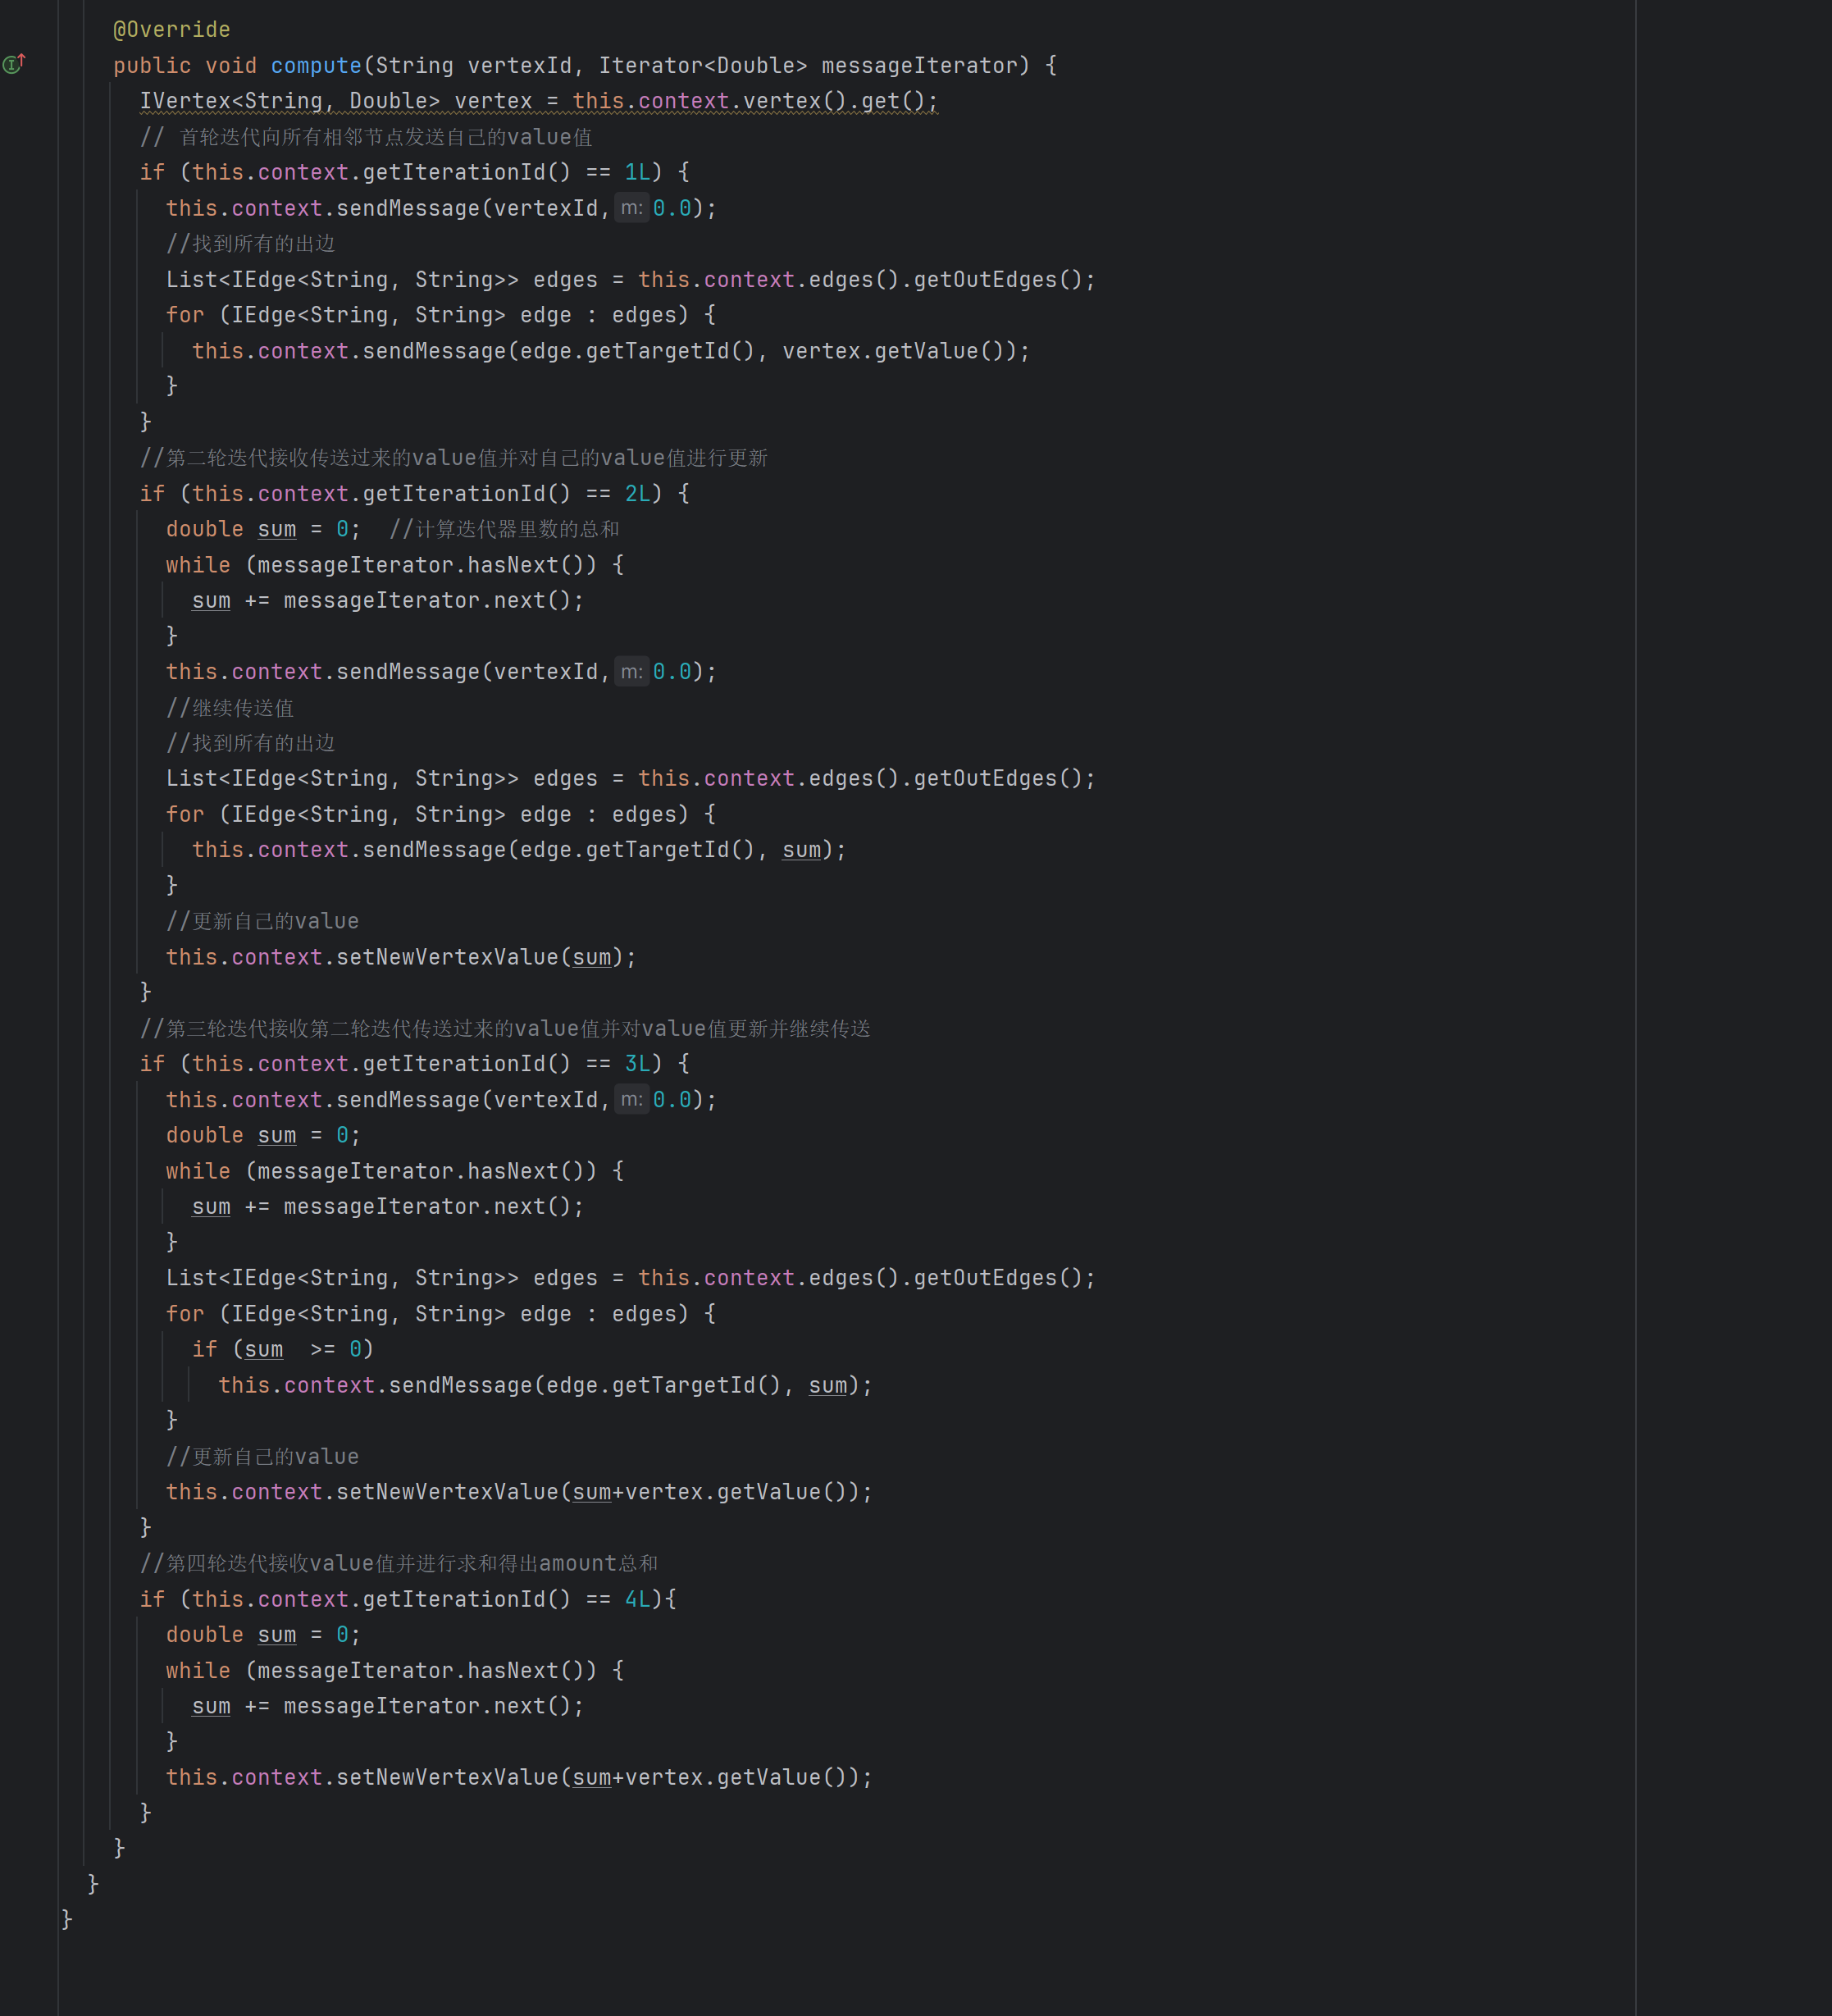
\includegraphics[width=0.85\textwidth,scale=0.7]{./figures/pro3/5.png}
  \end{center}
\end{figure}

最后将结果保存到文件中
\begin{figure}[H]
  \begin{center}
    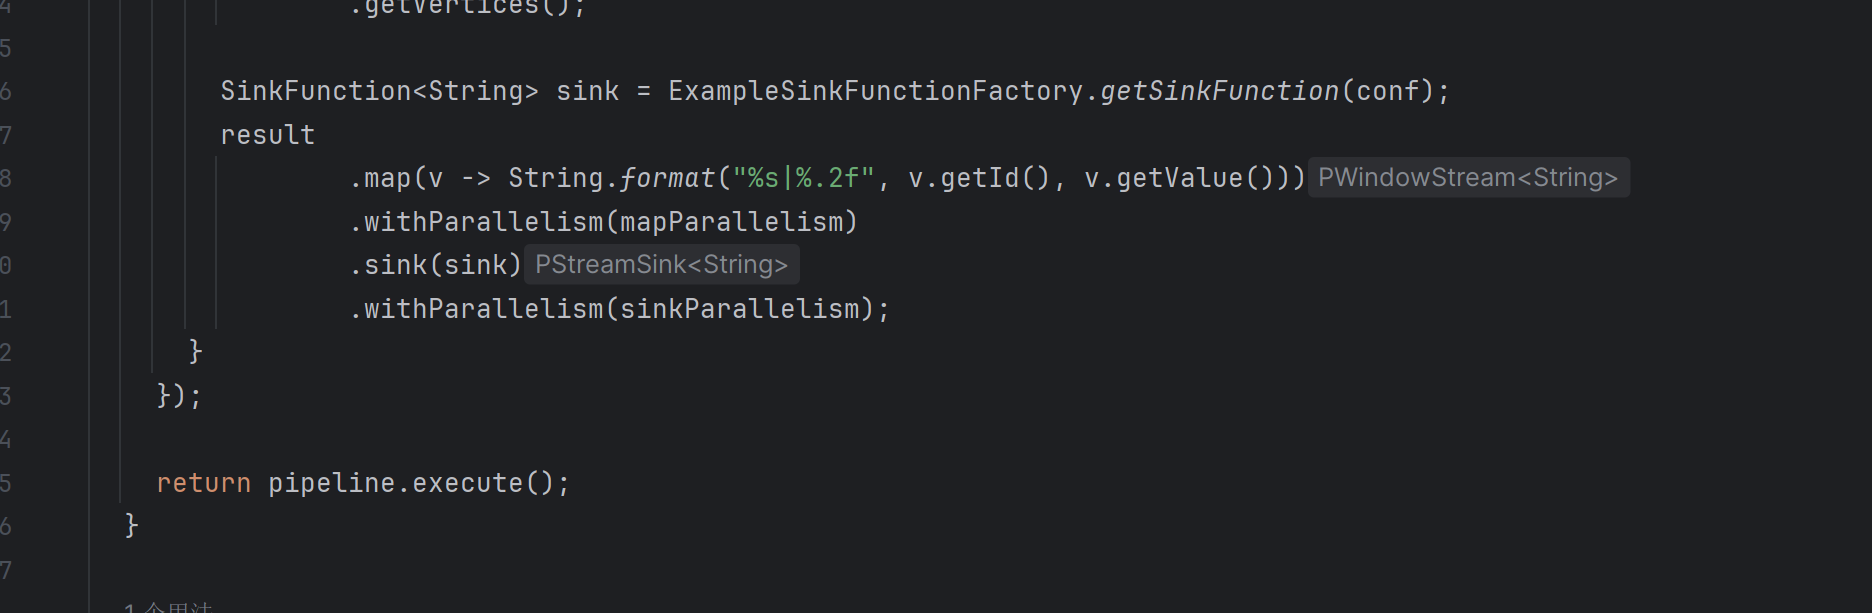
\includegraphics[width=0.85\textwidth,scale=0.7]{./figures/pro3/6.png}
  \end{center}
\end{figure}

但是,提交结果以失败告终了,经过分析,我们发现这个算法不能处理环的问题,因为如
果图中存在环,那么有的点的value值就会就会计算两遍。

\subsubsection{尝试代码优化改进}
上面的算法存在问题,所有我们进行思考后,决定改进第二步操作的compute算法,我们
将点封装成对象,并在迭代中将传递的数据类型改为string类型,可以来判断发送点的具体
信息,用set可以进行点的去重,判断发送源点是否已经给自己发送过数据。每个点首轮
向邻居发送一个消息(点id,1,0.00),当一个点收到消息后若消息的第二个元素
为1或2则直接给消息第一个元素对应的点发送自己的value并将第二个元素加1
传递给邻居;若第二个元素为3,则发送value而不继续传递;最后第二个元素
为4的就是担保链上所有的点发来的消息。
点的类描述如下:
\begin{figure}[H]
  \begin{center}
    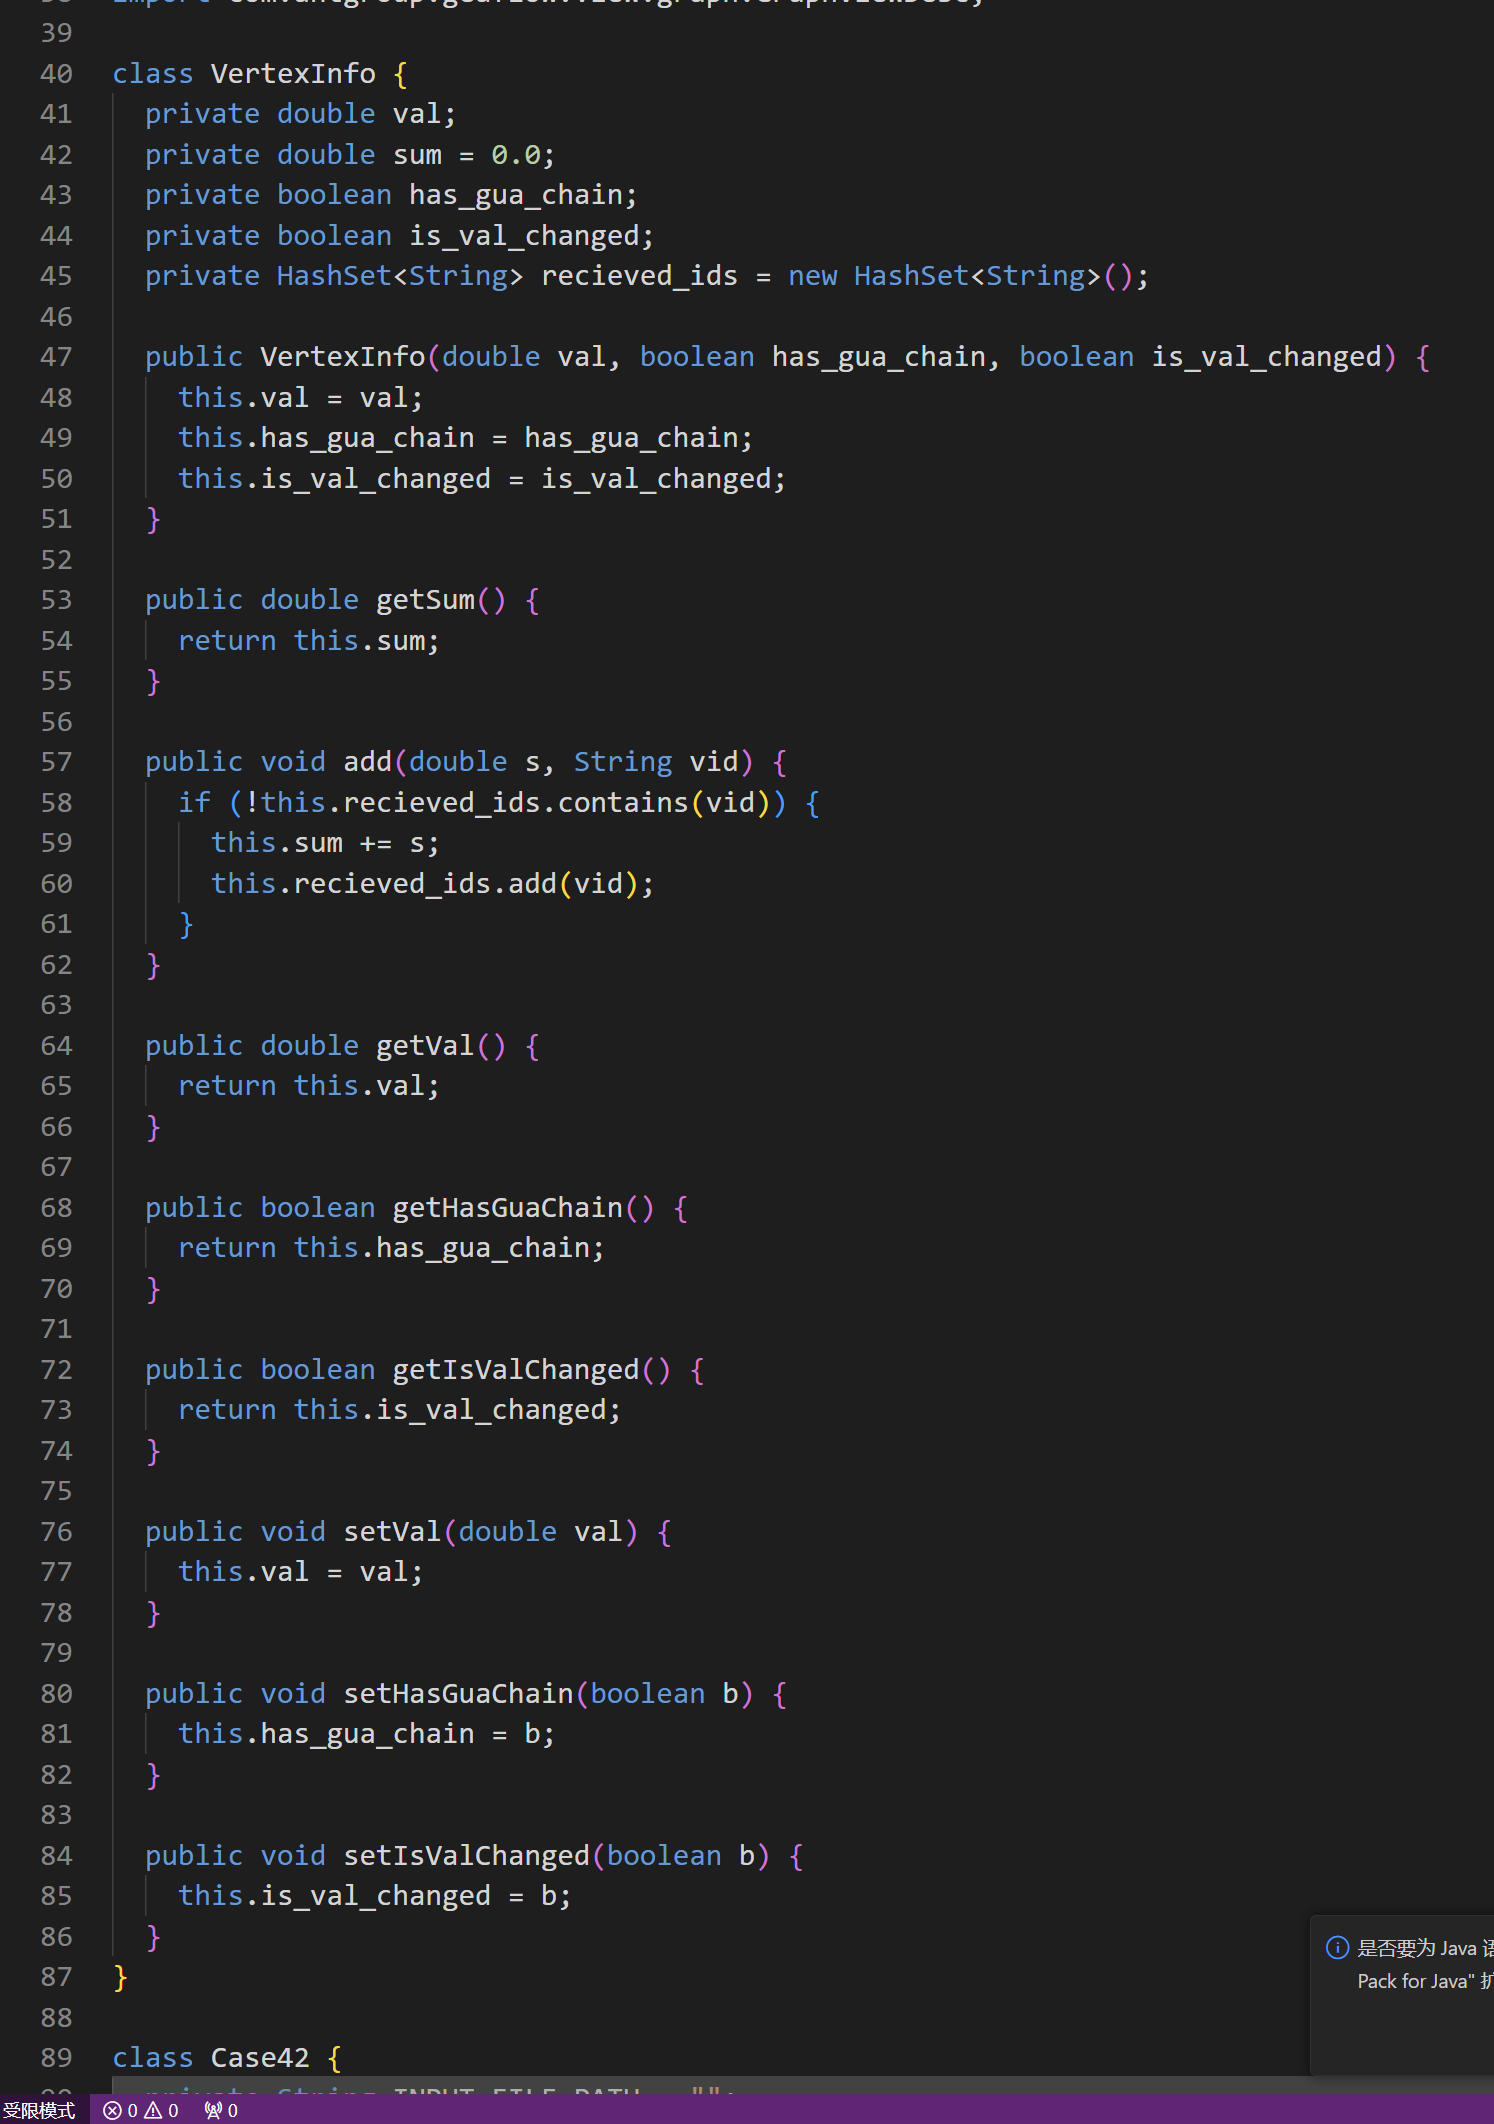
\includegraphics[width=0.85\textwidth,scale=0.7]{./figures/pro3/7.png}
  \end{center}
\end{figure}

更新后的compute如下:
\newpage

\begin{figure}[H]
  \begin{center}
    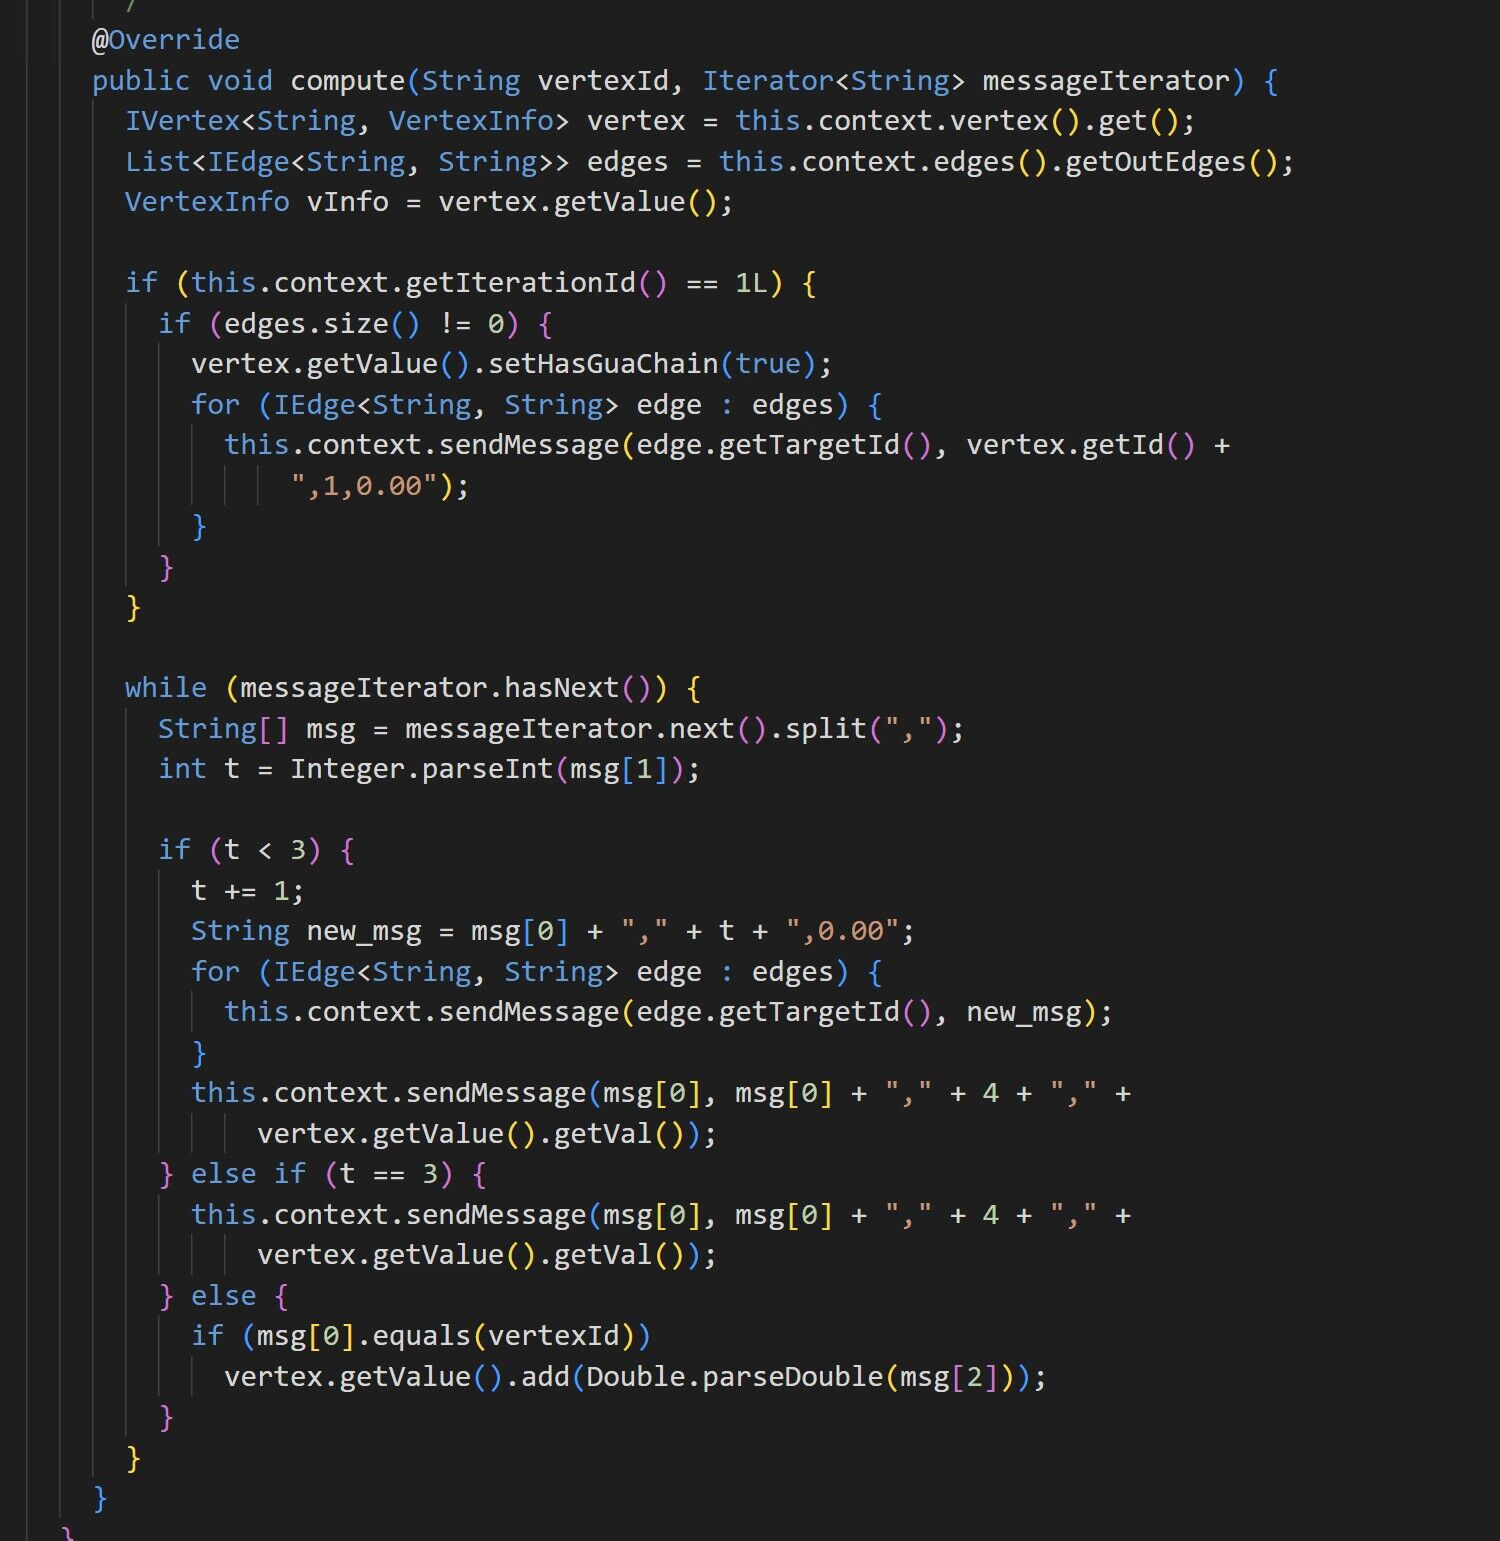
\includegraphics[width=0.55\textwidth,scale=0.5]{./figures/pro3/8.png}
  \end{center}
\end{figure}

我们尝试自己创建文件将自己能想到的所有情况进行测试,结果均正确。但是依然过不了
测试,宣告本题以失败告终。但是在尝试过程中也收获了许多知识点。

\subsection{个人贷款统计问题}
具体问题描述可见 \ref{pro4} 个人贷款统计问题一节.

备注:此case1我们花了一定时间,没有通过评测。最初其结果集有误,后续赛事组才进行
修改,我们当时忙于处理case4,遂对该题没有过多的深入。

此问题涉及的数据文件有:
\begin{itemize}
  \item Person.csv(点)
  \item Account.csv(点)
  \item Loan.csv(点)
  \item AccountTransferAccount.csv(边)
  \item LoanDepositAccount.csv(边)
  \item PersonOwnAccount.csv(边)
\end{itemize}

\subsubsection{思路历程}
根据题目需分三步走,逐步将loan值往前传。首先导入account点和loan点,
通过loandepositaccount的边和其值amout创建一张图,向前传递amount值;再将上一步
生成的含有accountid和value的表与accounttransferaccount的边结合生成一张图,将value
的值向前传递;最后将上一步生成的含有accountid和value的表与personownaccount边、
person点相结合,向前传递value值实现个人贷款的汇总。

\subsubsection{代码分析与实现}
运用赛题所给的接口,我们先将account和loan都当作点,点的id即为account或loan对应
的id,将account的初始value设为0,将loan的初始value设为-1(方便后续筛选);而对
于边,我们将loandepositaccount的amount设为其边的value,两侧点按顺序填入相应的id,
通过输入流pwindowsource分别进行输入。接着我们用buildwindowstreamgraph进行构图,
在构图中我们用union操作将loan和account点合并在一起。考虑到loan和account的id有重
复的部分(通过set检测,遍历两个文件后统计数量是否变化),由于loan点在后续代码中
并没有使用,因此在loan点的id前加入字符“l”以进行区分,防止account之间或者loan
之间的相连。代码如下:
\begin{figure}[H]
  \begin{center}
    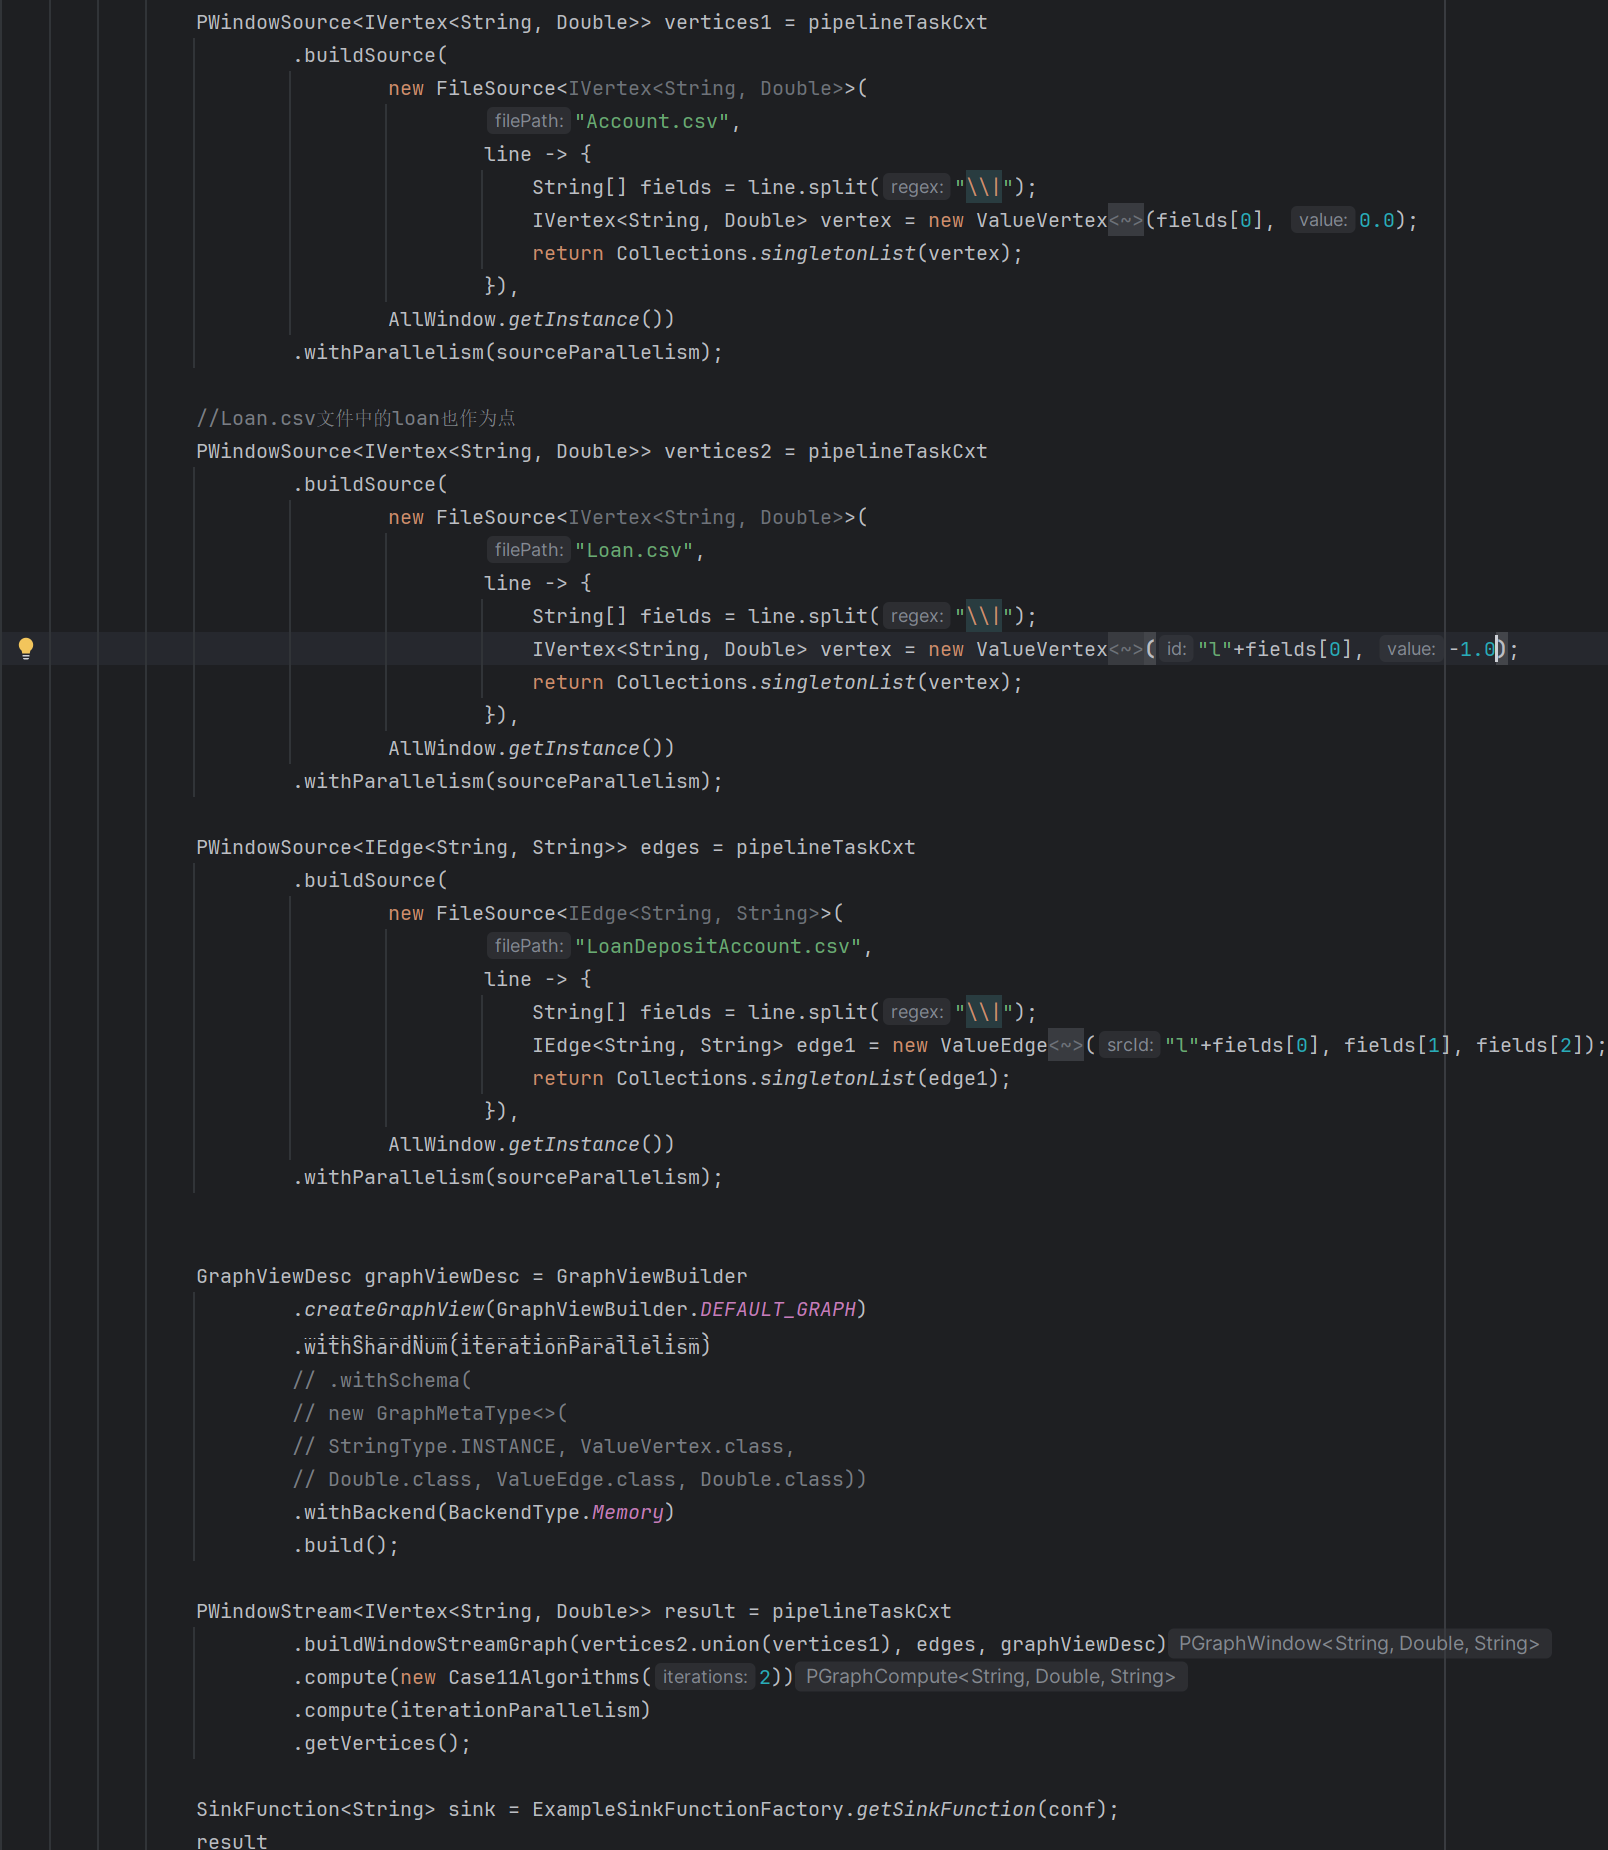
\includegraphics[width=0.85\textwidth,scale=0.7]{./figures/pro4/1.png}
  \end{center}
\end{figure}

接着我们需要得出一个新文件让每个account带上amount,于是,算法思路是进行对所有
点进行两轮迭代,第一轮所有点迭代中,让所有拥有出边的loan点(即此loan有至少一个
账户deposit),向所有出边的目标点(即account点)发送边的amount值。在第二轮迭代
中,由于每个点都有一个接收器,我们让所有接收器不为空的点计算接收器的总和sum并
将value值更新为sum,
到这一步,所有account的value值大于等于 $ 0 $,所有loan的value值都为 $ -1 $,核心代码如下:
\begin{figure}[H]
  \begin{center}
    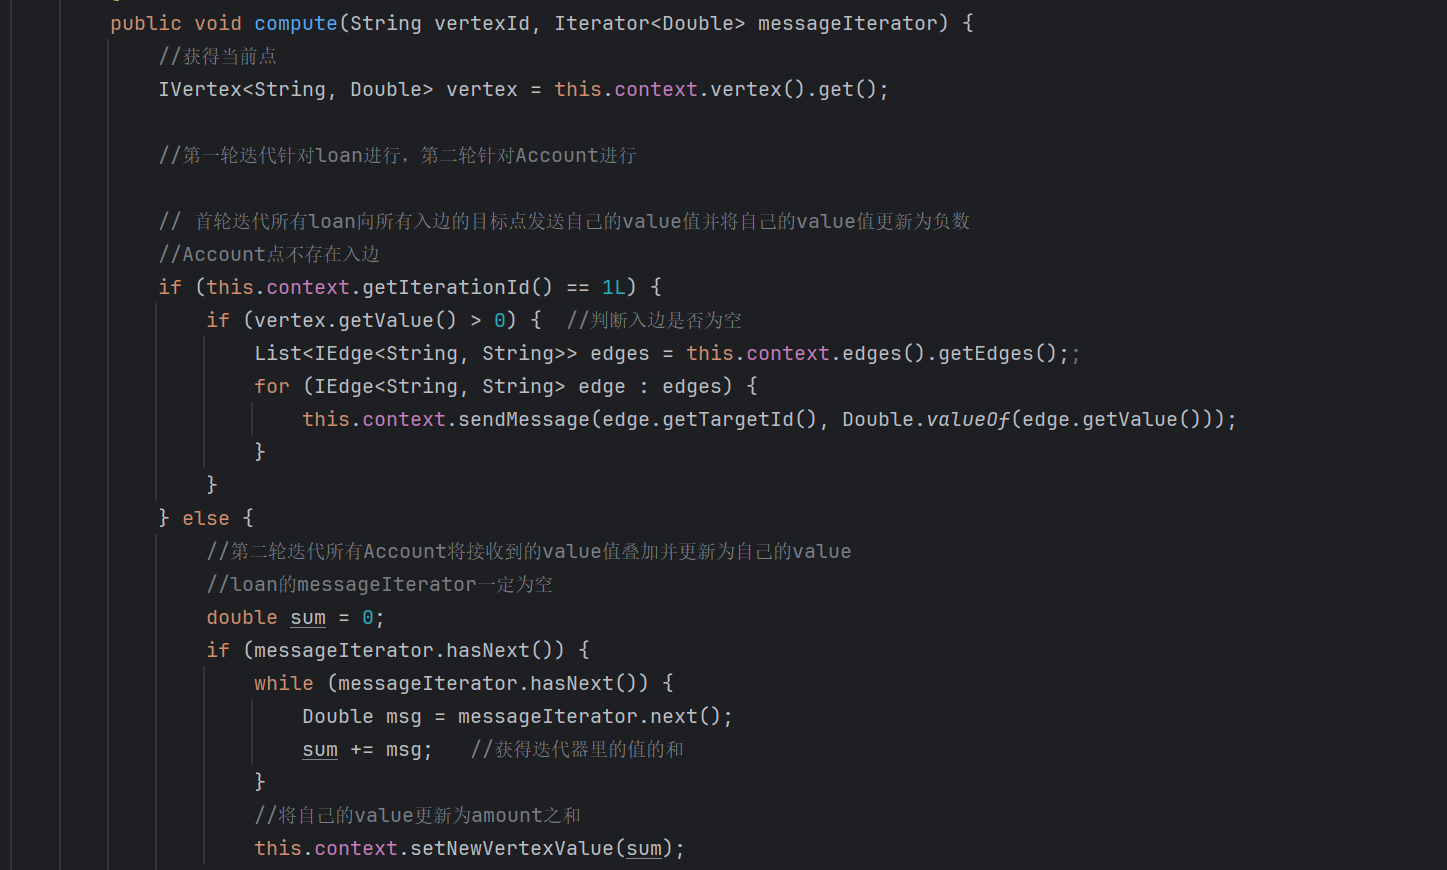
\includegraphics[width=0.85\textwidth,scale=0.7]{./figures/pro4/2.png}
  \end{center}
\end{figure}

最后,将所有点进行过滤涤除value 小于 $ 0 $ 的点(即loan点)得到中间文件。
\begin{figure}[H]
  \begin{center}
    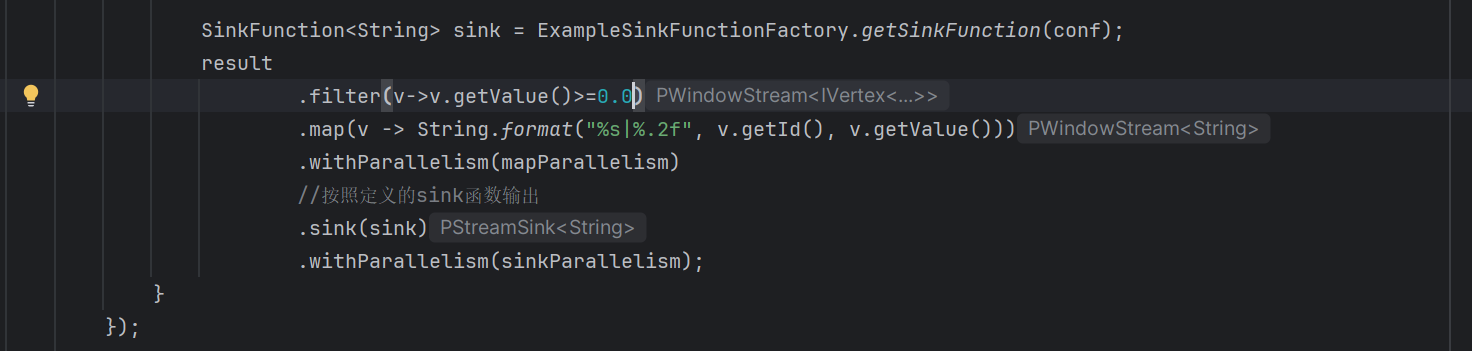
\includegraphics[width=0.85\textwidth,scale=0.7]{./figures/pro4/3.png}
  \end{center}
\end{figure}

接着进入第二步操作,首先我们将中间文件与accounttransferaccount文件联合起来构建成
图,点的id为account的id,点的value为account的value,边的value为空字符串:
\begin{figure}[H]
  \begin{center}
    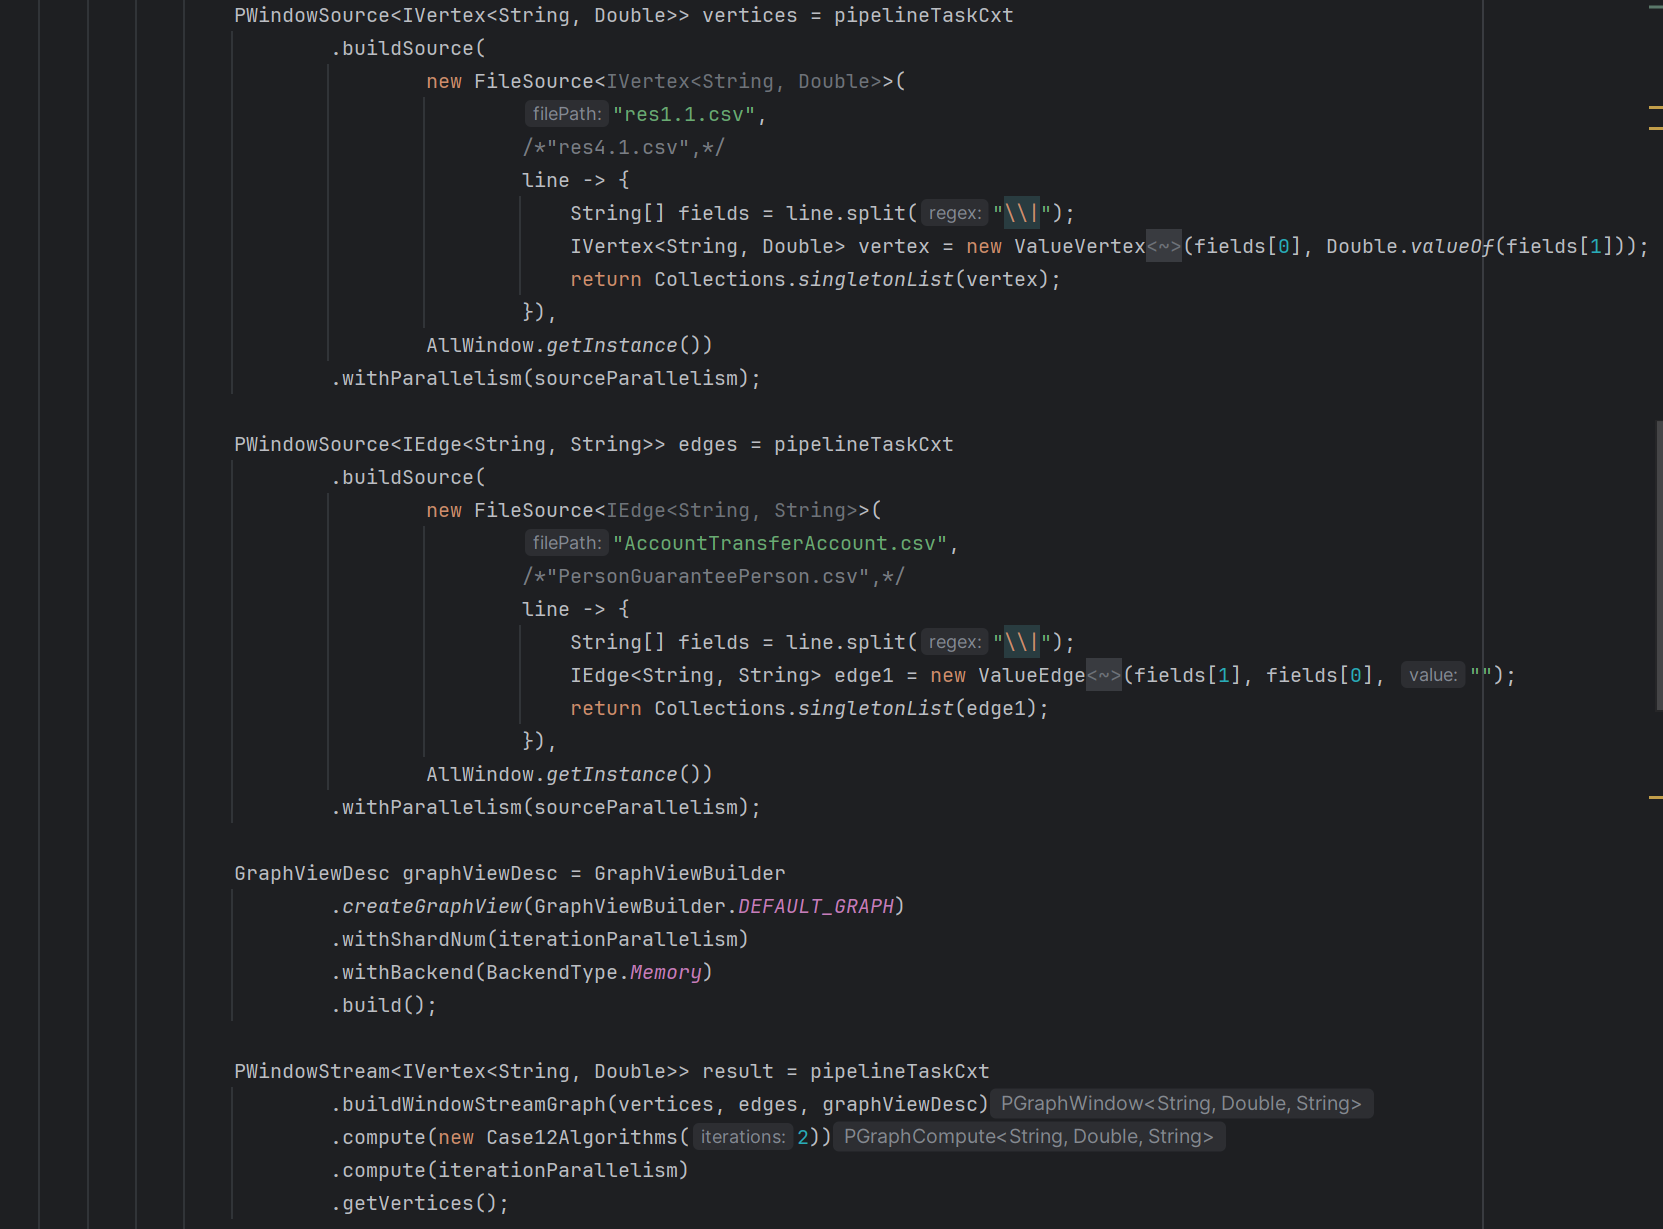
\includegraphics[width=0.85\textwidth,scale=0.7]{./figures/pro4/4.png}
  \end{center}
\end{figure}

接着我们进行两轮迭代,与第一次处理类似,将点的value值根据边往前传递。
需要注意的是,为防止未经过transfer的点在最后一轮也被计算进去,在传递前先让所有点
都向自己的接收器发送0.0(接收器没有值的点不会进入第二轮迭代),并在第二轮迭代中
进行更新value值,这样就只有通过边传递值的account的value值不为0。核心代码如下:
\begin{figure}[H]
  \begin{center}
    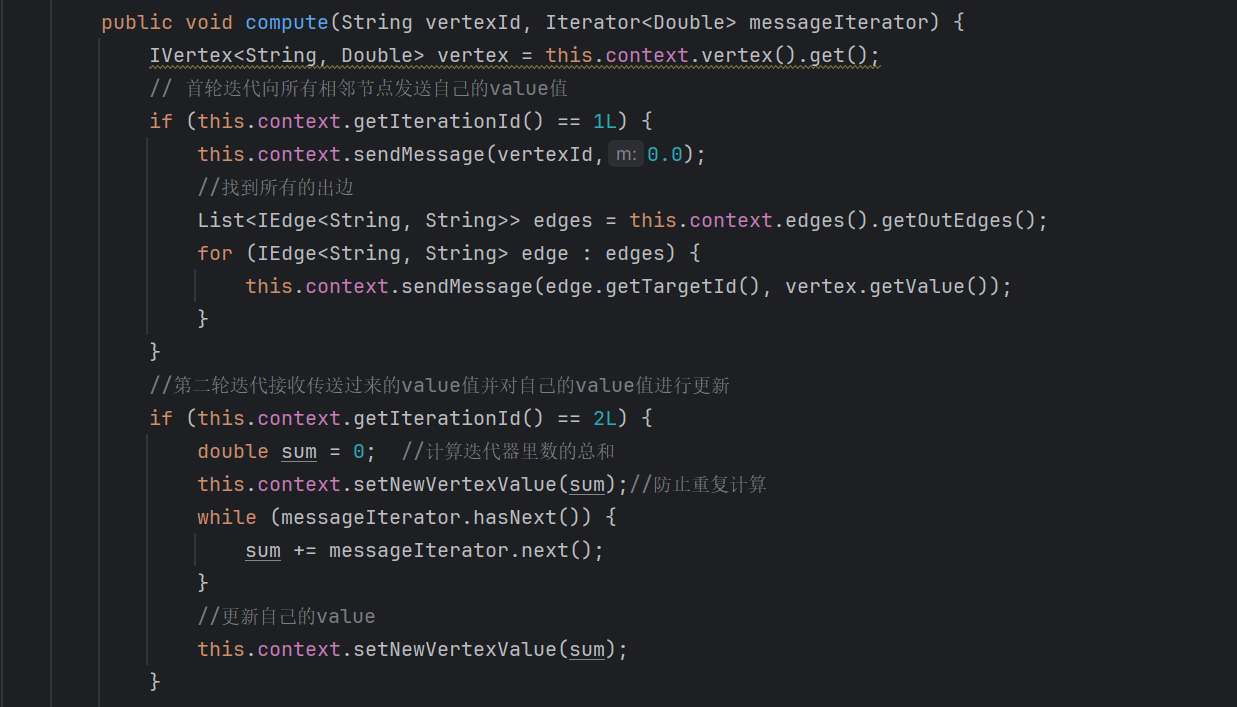
\includegraphics[width=0.85\textwidth,scale=0.7]{./figures/pro4/5.png}
  \end{center}
\end{figure}

第二次中间文件输出格式如下:
\begin{figure}[H]
  \begin{center}
    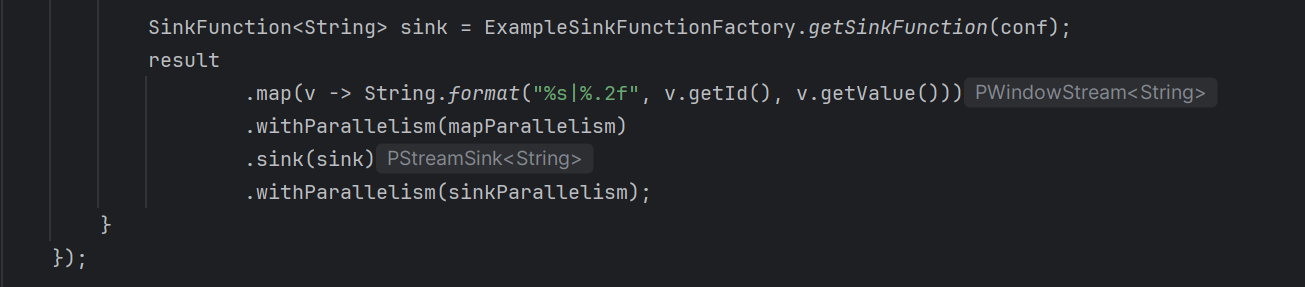
\includegraphics[width=0.85\textwidth,scale=0.7]{./figures/pro4/6.png}
  \end{center}
\end{figure}

接着进入第三步操作,首先我们将中间文件与personownaccount文件和person文件联合起
来构建成图,点的id为account或者person的id,点的value为account的value,person的
value置为0,边的value为空字符串:
\begin{figure}[H]
  \begin{center}
    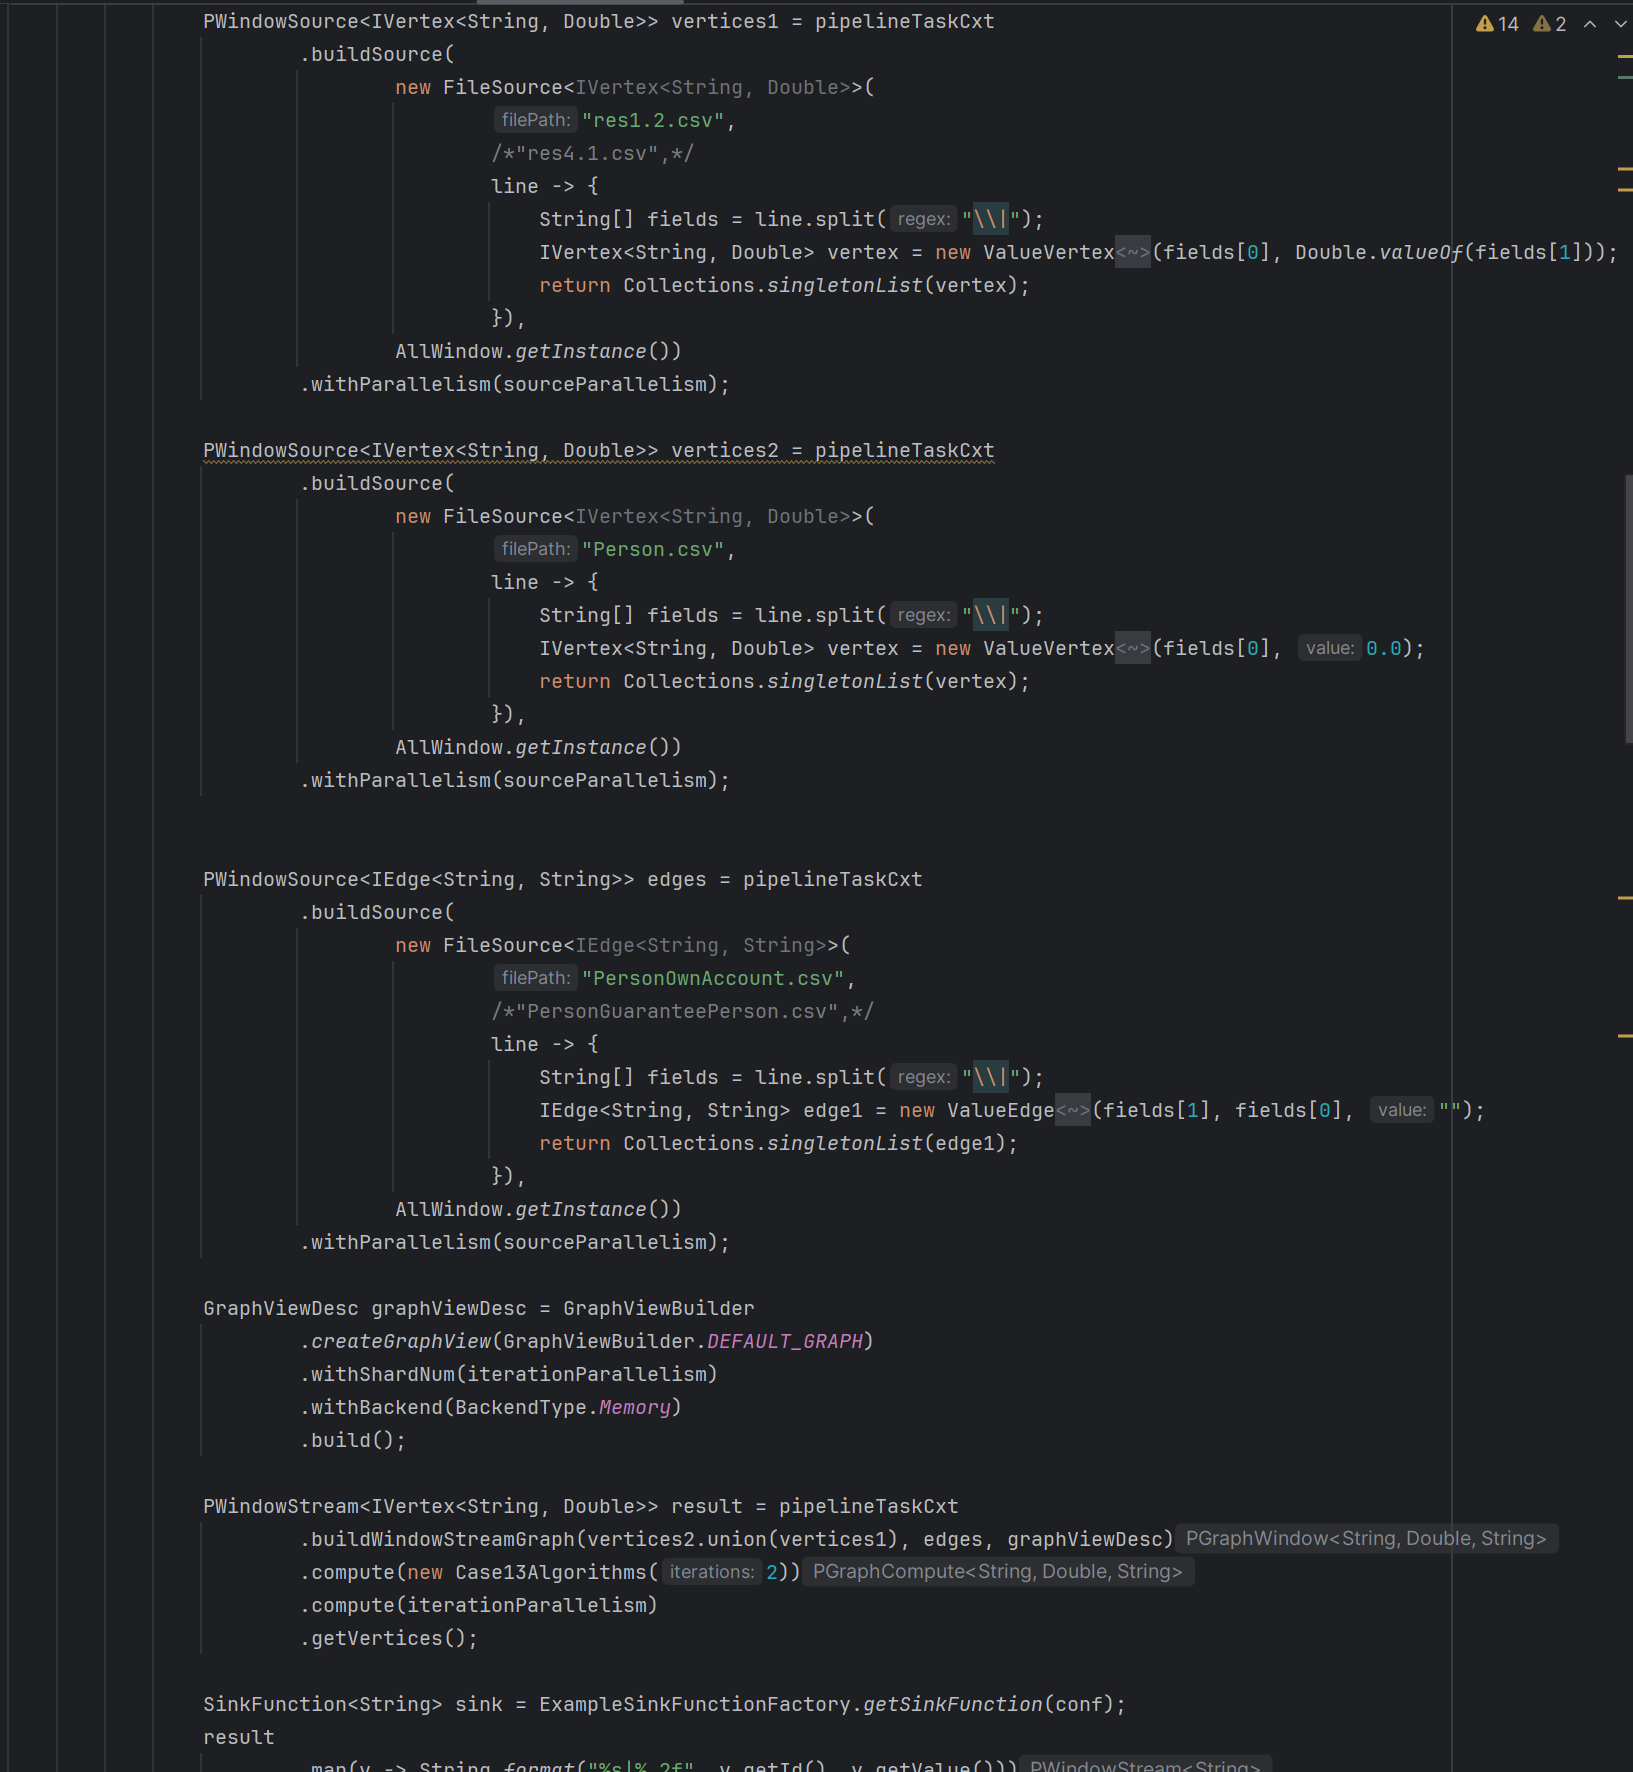
\includegraphics[width=0.85\textwidth,scale=0.7]{./figures/pro4/7.png}
  \end{center}
\end{figure}

接着我们进行两轮迭代,与第二次处理类似,将点的value值根据边往前传递。
不过这次将所有点发送的值为 $ -1 $,用于后续将account点筛选掉。核心代码如下:
\begin{figure}[H]
  \begin{center}
    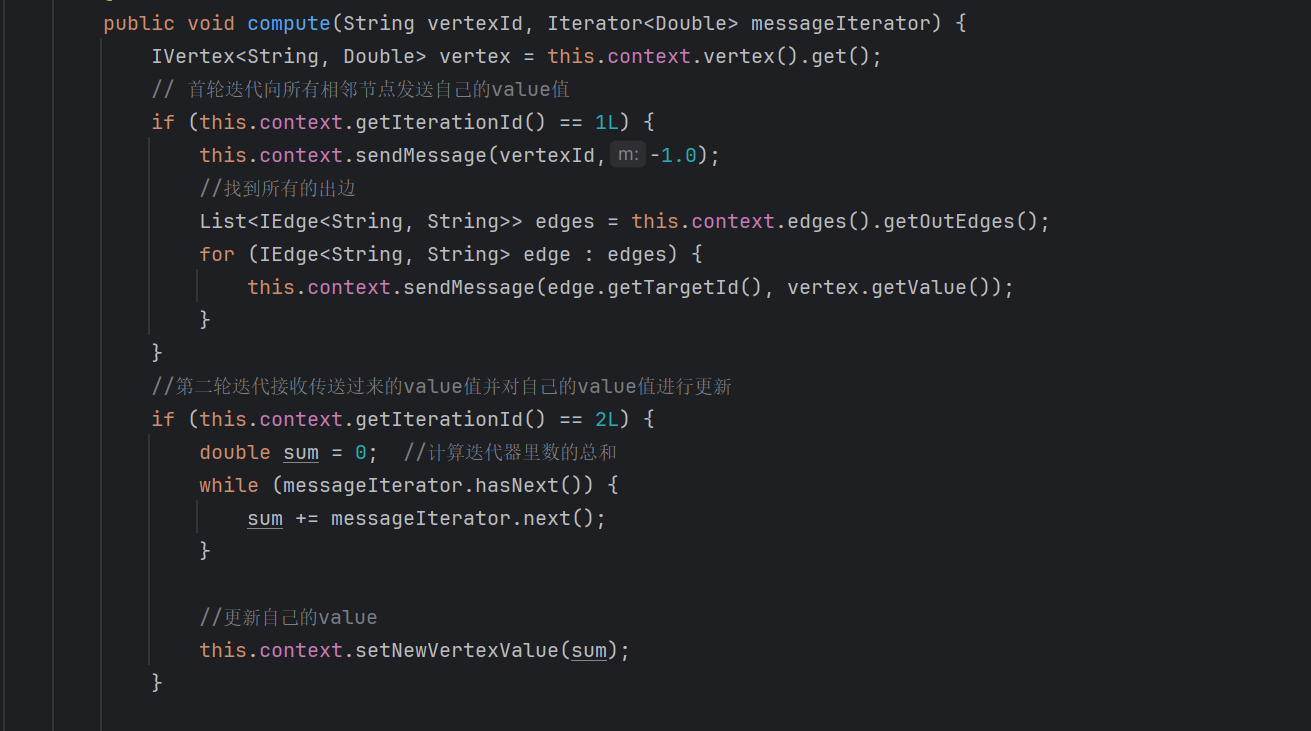
\includegraphics[width=0.85\textwidth,scale=0.7]{./figures/pro4/8.png}
  \end{center}
\end{figure}

最后将结果后保存到文件中
\begin{figure}[H]
  \begin{center}
    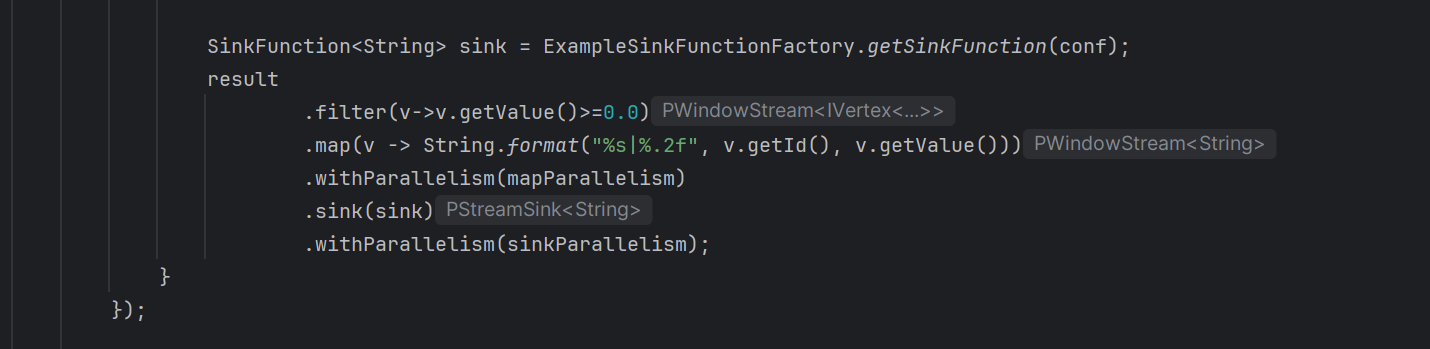
\includegraphics[width=0.85\textwidth,scale=0.7]{./figures/pro4/9.png}
  \end{center}
\end{figure}

但是,提交结果以失败告终了。
我们尝试自己创建文件将自己能想到的所有情况进行测试,结果均正确。但是依然过不了测试,宣告本题以失败告终。但是在尝试过程中也收获了许多知识点。

